\documentclass[]{article}
\usepackage{lmodern}
\usepackage{amssymb,amsmath}
\usepackage{ifxetex,ifluatex}
\usepackage{fixltx2e} % provides \textsubscript
\ifnum 0\ifxetex 1\fi\ifluatex 1\fi=0 % if pdftex
  \usepackage[T1]{fontenc}
  \usepackage[utf8]{inputenc}
\else % if luatex or xelatex
  \ifxetex
    \usepackage{mathspec}
  \else
    \usepackage{fontspec}
  \fi
  \defaultfontfeatures{Ligatures=TeX,Scale=MatchLowercase}
\fi
% use upquote if available, for straight quotes in verbatim environments
\IfFileExists{upquote.sty}{\usepackage{upquote}}{}
% use microtype if available
\IfFileExists{microtype.sty}{%
\usepackage{microtype}
\UseMicrotypeSet[protrusion]{basicmath} % disable protrusion for tt fonts
}{}
\usepackage[margin=1in]{geometry}
\usepackage{hyperref}
\hypersetup{unicode=true,
            pdftitle={Mixture Models},
            pdfauthor={Abdul-Rahman},
            pdfborder={0 0 0},
            breaklinks=true}
\urlstyle{same}  % don't use monospace font for urls
\usepackage{color}
\usepackage{fancyvrb}
\newcommand{\VerbBar}{|}
\newcommand{\VERB}{\Verb[commandchars=\\\{\}]}
\DefineVerbatimEnvironment{Highlighting}{Verbatim}{commandchars=\\\{\}}
% Add ',fontsize=\small' for more characters per line
\usepackage{framed}
\definecolor{shadecolor}{RGB}{248,248,248}
\newenvironment{Shaded}{\begin{snugshade}}{\end{snugshade}}
\newcommand{\AlertTok}[1]{\textcolor[rgb]{0.94,0.16,0.16}{#1}}
\newcommand{\AnnotationTok}[1]{\textcolor[rgb]{0.56,0.35,0.01}{\textbf{\textit{#1}}}}
\newcommand{\AttributeTok}[1]{\textcolor[rgb]{0.77,0.63,0.00}{#1}}
\newcommand{\BaseNTok}[1]{\textcolor[rgb]{0.00,0.00,0.81}{#1}}
\newcommand{\BuiltInTok}[1]{#1}
\newcommand{\CharTok}[1]{\textcolor[rgb]{0.31,0.60,0.02}{#1}}
\newcommand{\CommentTok}[1]{\textcolor[rgb]{0.56,0.35,0.01}{\textit{#1}}}
\newcommand{\CommentVarTok}[1]{\textcolor[rgb]{0.56,0.35,0.01}{\textbf{\textit{#1}}}}
\newcommand{\ConstantTok}[1]{\textcolor[rgb]{0.00,0.00,0.00}{#1}}
\newcommand{\ControlFlowTok}[1]{\textcolor[rgb]{0.13,0.29,0.53}{\textbf{#1}}}
\newcommand{\DataTypeTok}[1]{\textcolor[rgb]{0.13,0.29,0.53}{#1}}
\newcommand{\DecValTok}[1]{\textcolor[rgb]{0.00,0.00,0.81}{#1}}
\newcommand{\DocumentationTok}[1]{\textcolor[rgb]{0.56,0.35,0.01}{\textbf{\textit{#1}}}}
\newcommand{\ErrorTok}[1]{\textcolor[rgb]{0.64,0.00,0.00}{\textbf{#1}}}
\newcommand{\ExtensionTok}[1]{#1}
\newcommand{\FloatTok}[1]{\textcolor[rgb]{0.00,0.00,0.81}{#1}}
\newcommand{\FunctionTok}[1]{\textcolor[rgb]{0.00,0.00,0.00}{#1}}
\newcommand{\ImportTok}[1]{#1}
\newcommand{\InformationTok}[1]{\textcolor[rgb]{0.56,0.35,0.01}{\textbf{\textit{#1}}}}
\newcommand{\KeywordTok}[1]{\textcolor[rgb]{0.13,0.29,0.53}{\textbf{#1}}}
\newcommand{\NormalTok}[1]{#1}
\newcommand{\OperatorTok}[1]{\textcolor[rgb]{0.81,0.36,0.00}{\textbf{#1}}}
\newcommand{\OtherTok}[1]{\textcolor[rgb]{0.56,0.35,0.01}{#1}}
\newcommand{\PreprocessorTok}[1]{\textcolor[rgb]{0.56,0.35,0.01}{\textit{#1}}}
\newcommand{\RegionMarkerTok}[1]{#1}
\newcommand{\SpecialCharTok}[1]{\textcolor[rgb]{0.00,0.00,0.00}{#1}}
\newcommand{\SpecialStringTok}[1]{\textcolor[rgb]{0.31,0.60,0.02}{#1}}
\newcommand{\StringTok}[1]{\textcolor[rgb]{0.31,0.60,0.02}{#1}}
\newcommand{\VariableTok}[1]{\textcolor[rgb]{0.00,0.00,0.00}{#1}}
\newcommand{\VerbatimStringTok}[1]{\textcolor[rgb]{0.31,0.60,0.02}{#1}}
\newcommand{\WarningTok}[1]{\textcolor[rgb]{0.56,0.35,0.01}{\textbf{\textit{#1}}}}
\usepackage{graphicx,grffile}
\makeatletter
\def\maxwidth{\ifdim\Gin@nat@width>\linewidth\linewidth\else\Gin@nat@width\fi}
\def\maxheight{\ifdim\Gin@nat@height>\textheight\textheight\else\Gin@nat@height\fi}
\makeatother
% Scale images if necessary, so that they will not overflow the page
% margins by default, and it is still possible to overwrite the defaults
% using explicit options in \includegraphics[width, height, ...]{}
\setkeys{Gin}{width=\maxwidth,height=\maxheight,keepaspectratio}
\IfFileExists{parskip.sty}{%
\usepackage{parskip}
}{% else
\setlength{\parindent}{0pt}
\setlength{\parskip}{6pt plus 2pt minus 1pt}
}
\setlength{\emergencystretch}{3em}  % prevent overfull lines
\providecommand{\tightlist}{%
  \setlength{\itemsep}{0pt}\setlength{\parskip}{0pt}}
\setcounter{secnumdepth}{0}
% Redefines (sub)paragraphs to behave more like sections
\ifx\paragraph\undefined\else
\let\oldparagraph\paragraph
\renewcommand{\paragraph}[1]{\oldparagraph{#1}\mbox{}}
\fi
\ifx\subparagraph\undefined\else
\let\oldsubparagraph\subparagraph
\renewcommand{\subparagraph}[1]{\oldsubparagraph{#1}\mbox{}}
\fi

%%% Use protect on footnotes to avoid problems with footnotes in titles
\let\rmarkdownfootnote\footnote%
\def\footnote{\protect\rmarkdownfootnote}

%%% Change title format to be more compact
\usepackage{titling}

% Create subtitle command for use in maketitle
\providecommand{\subtitle}[1]{
  \posttitle{
    \begin{center}\large#1\end{center}
    }
}

\setlength{\droptitle}{-2em}

  \title{Mixture Models}
    \pretitle{\vspace{\droptitle}\centering\huge}
  \posttitle{\par}
    \author{Abdul-Rahman}
    \preauthor{\centering\large\emph}
  \postauthor{\par}
      \predate{\centering\large\emph}
  \postdate{\par}
    \date{10/10/2019}


\begin{document}
\maketitle

\begin{Shaded}
\begin{Highlighting}[]
\KeywordTok{library}\NormalTok{(}\StringTok{"ggplot2"}\NormalTok{)}
\KeywordTok{library}\NormalTok{(}\StringTok{"dplyr"}\NormalTok{)}
\end{Highlighting}
\end{Shaded}

\begin{verbatim}
## 
## Attaching package: 'dplyr'
\end{verbatim}

\begin{verbatim}
## The following objects are masked from 'package:stats':
## 
##     filter, lag
\end{verbatim}

\begin{verbatim}
## The following objects are masked from 'package:base':
## 
##     intersect, setdiff, setequal, union
\end{verbatim}

\begin{Shaded}
\begin{Highlighting}[]
\KeywordTok{library}\NormalTok{(}\StringTok{"mixtools"}\NormalTok{)}
\end{Highlighting}
\end{Shaded}

\begin{verbatim}
## mixtools package, version 1.1.0, Released 2017-03-10
## This package is based upon work supported by the National Science Foundation under Grant No. SES-0518772.
\end{verbatim}

\begin{Shaded}
\begin{Highlighting}[]
\KeywordTok{library}\NormalTok{(}\StringTok{"mosaics"}\NormalTok{)}
\end{Highlighting}
\end{Shaded}

\begin{verbatim}
## Loading required package: Rcpp
\end{verbatim}

\begin{Shaded}
\begin{Highlighting}[]
\KeywordTok{library}\NormalTok{(}\StringTok{"mosaicsExample"}\NormalTok{)}
\KeywordTok{library}\NormalTok{(}\StringTok{"HistData"}\NormalTok{)}
\KeywordTok{library}\NormalTok{(}\StringTok{"bootstrap"}\NormalTok{)}
\KeywordTok{library}\NormalTok{(}\StringTok{"ggbeeswarm"}\NormalTok{)}
\KeywordTok{library}\NormalTok{(}\StringTok{"RColorBrewer"}\NormalTok{)  }
\KeywordTok{library}\NormalTok{(}\StringTok{"ggthemes"}\NormalTok{)  }
\KeywordTok{library}\NormalTok{(}\StringTok{"magrittr"}\NormalTok{)  }
\KeywordTok{library}\NormalTok{(}\StringTok{"plotly"}\NormalTok{)  }
\end{Highlighting}
\end{Shaded}

\begin{verbatim}
## 
## Attaching package: 'plotly'
\end{verbatim}

\begin{verbatim}
## The following object is masked from 'package:mosaics':
## 
##     export
\end{verbatim}

\begin{verbatim}
## The following object is masked from 'package:ggplot2':
## 
##     last_plot
\end{verbatim}

\begin{verbatim}
## The following object is masked from 'package:stats':
## 
##     filter
\end{verbatim}

\begin{verbatim}
## The following object is masked from 'package:graphics':
## 
##     layout
\end{verbatim}

\begin{Shaded}
\begin{Highlighting}[]
\KeywordTok{library}\NormalTok{(}\StringTok{"pheatmap"}\NormalTok{)  }
\KeywordTok{library}\NormalTok{(}\StringTok{"colorspace"}\NormalTok{)  }
\KeywordTok{library}\NormalTok{(}\StringTok{"grid"}\NormalTok{)  }
\end{Highlighting}
\end{Shaded}

\begin{verbatim}
## 
## Attaching package: 'grid'
\end{verbatim}

\begin{verbatim}
## The following object is masked from 'package:mixtools':
## 
##     depth
\end{verbatim}

\begin{Shaded}
\begin{Highlighting}[]
\KeywordTok{library}\NormalTok{(}\StringTok{"ggbio"}\NormalTok{) }
\end{Highlighting}
\end{Shaded}

\begin{verbatim}
## Loading required package: BiocGenerics
\end{verbatim}

\begin{verbatim}
## Loading required package: parallel
\end{verbatim}

\begin{verbatim}
## 
## Attaching package: 'BiocGenerics'
\end{verbatim}

\begin{verbatim}
## The following objects are masked from 'package:parallel':
## 
##     clusterApply, clusterApplyLB, clusterCall, clusterEvalQ,
##     clusterExport, clusterMap, parApply, parCapply, parLapply,
##     parLapplyLB, parRapply, parSapply, parSapplyLB
\end{verbatim}

\begin{verbatim}
## The following objects are masked from 'package:dplyr':
## 
##     combine, intersect, setdiff, union
\end{verbatim}

\begin{verbatim}
## The following objects are masked from 'package:stats':
## 
##     IQR, mad, sd, var, xtabs
\end{verbatim}

\begin{verbatim}
## The following objects are masked from 'package:base':
## 
##     anyDuplicated, append, as.data.frame, basename, cbind,
##     colnames, dirname, do.call, duplicated, eval, evalq, Filter,
##     Find, get, grep, grepl, intersect, is.unsorted, lapply, Map,
##     mapply, match, mget, order, paste, pmax, pmax.int, pmin,
##     pmin.int, Position, rank, rbind, Reduce, rownames, sapply,
##     setdiff, sort, table, tapply, union, unique, unsplit, which,
##     which.max, which.min
\end{verbatim}

\begin{verbatim}
## Registered S3 method overwritten by 'GGally':
##   method from   
##   +.gg   ggplot2
\end{verbatim}

\begin{verbatim}
## Need specific help about ggbio? try mailing 
##  the maintainer or visit http://tengfei.github.com/ggbio/
\end{verbatim}

\begin{verbatim}
## 
## Attaching package: 'ggbio'
\end{verbatim}

\begin{verbatim}
## The following objects are masked from 'package:ggplot2':
## 
##     geom_bar, geom_rect, geom_segment, ggsave, stat_bin,
##     stat_identity, xlim
\end{verbatim}

\begin{Shaded}
\begin{Highlighting}[]
\KeywordTok{library}\NormalTok{(GenomicRanges)}
\end{Highlighting}
\end{Shaded}

\begin{verbatim}
## Loading required package: stats4
\end{verbatim}

\begin{verbatim}
## Loading required package: S4Vectors
\end{verbatim}

\begin{verbatim}
## 
## Attaching package: 'S4Vectors'
\end{verbatim}

\begin{verbatim}
## The following object is masked from 'package:plotly':
## 
##     rename
\end{verbatim}

\begin{verbatim}
## The following objects are masked from 'package:dplyr':
## 
##     first, rename
\end{verbatim}

\begin{verbatim}
## The following object is masked from 'package:base':
## 
##     expand.grid
\end{verbatim}

\begin{verbatim}
## Loading required package: IRanges
\end{verbatim}

\begin{verbatim}
## 
## Attaching package: 'IRanges'
\end{verbatim}

\begin{verbatim}
## The following object is masked from 'package:plotly':
## 
##     slice
\end{verbatim}

\begin{verbatim}
## The following objects are masked from 'package:dplyr':
## 
##     collapse, desc, slice
\end{verbatim}

\begin{verbatim}
## Loading required package: GenomeInfoDb
\end{verbatim}

\begin{Shaded}
\begin{Highlighting}[]
\KeywordTok{library}\NormalTok{(}\StringTok{"flexmix"}\NormalTok{)}
\end{Highlighting}
\end{Shaded}

\begin{verbatim}
## Loading required package: lattice
\end{verbatim}

\begin{Shaded}
\begin{Highlighting}[]
\KeywordTok{library}\NormalTok{(}\StringTok{"mclust"}\NormalTok{)}
\end{Highlighting}
\end{Shaded}

\begin{verbatim}
## Package 'mclust' version 5.4.5
## Type 'citation("mclust")' for citing this R package in publications.
\end{verbatim}

\begin{verbatim}
## 
## Attaching package: 'mclust'
\end{verbatim}

\begin{verbatim}
## The following object is masked from 'package:bootstrap':
## 
##     diabetes
\end{verbatim}

\begin{verbatim}
## The following object is masked from 'package:mixtools':
## 
##     dmvnorm
\end{verbatim}

\begin{Shaded}
\begin{Highlighting}[]
\KeywordTok{library}\NormalTok{(}\StringTok{"mixtools"}\NormalTok{)}
\KeywordTok{library}\NormalTok{(}\StringTok{"mosaics"}\NormalTok{)}
\KeywordTok{library}\NormalTok{(}\StringTok{"mosaicsExample"}\NormalTok{)}
\KeywordTok{library}\NormalTok{(}\StringTok{"here"}\NormalTok{)}
\end{Highlighting}
\end{Shaded}

\begin{verbatim}
## here() starts at /Users/abdul-rahmanbukari/Documents/BIOSTATS
\end{verbatim}

\begin{Shaded}
\begin{Highlighting}[]
\KeywordTok{library}\NormalTok{(HistData)}
\KeywordTok{library}\NormalTok{(bootstrap)}
\KeywordTok{library}\NormalTok{(vcd)}
\end{Highlighting}
\end{Shaded}

\begin{verbatim}
## 
## Attaching package: 'vcd'
\end{verbatim}

\begin{verbatim}
## The following object is masked from 'package:GenomicRanges':
## 
##     tile
\end{verbatim}

\begin{verbatim}
## The following object is masked from 'package:IRanges':
## 
##     tile
\end{verbatim}

\hypertarget{finite-mixtures}{%
\subsection{Finite Mixtures}\label{finite-mixtures}}

Generate a random number from a normal distribution with mean 3 and
variance 0.25

\begin{Shaded}
\begin{Highlighting}[]
\KeywordTok{set.seed}\NormalTok{(}\DecValTok{1234}\NormalTok{)}
\NormalTok{coinflips =}\StringTok{ }\NormalTok{(}\KeywordTok{runif}\NormalTok{(}\DecValTok{10000}\NormalTok{) }\OperatorTok{>}\StringTok{ }\FloatTok{0.5}\NormalTok{)}
\KeywordTok{table}\NormalTok{(coinflips)}
\end{Highlighting}
\end{Shaded}

\begin{verbatim}
## coinflips
## FALSE  TRUE 
##  4990  5010
\end{verbatim}

\begin{Shaded}
\begin{Highlighting}[]
\NormalTok{oneFlip =}\StringTok{ }\ControlFlowTok{function}\NormalTok{(fl, }\DataTypeTok{mean1 =} \DecValTok{1}\NormalTok{, }\DataTypeTok{mean2 =} \DecValTok{3}\NormalTok{, }\DataTypeTok{sd1 =} \FloatTok{0.5}\NormalTok{, }\DataTypeTok{sd2 =} \FloatTok{0.5}\NormalTok{) \{}
  \ControlFlowTok{if}\NormalTok{ (fl) \{}
   \KeywordTok{rnorm}\NormalTok{(}\DecValTok{1}\NormalTok{, mean1, sd1)}
\NormalTok{  \} }\ControlFlowTok{else}\NormalTok{ \{}
   \KeywordTok{rnorm}\NormalTok{(}\DecValTok{1}\NormalTok{, mean2, sd2)}
\NormalTok{  \}}
\NormalTok{\}}
\NormalTok{fairmix =}\StringTok{ }\KeywordTok{vapply}\NormalTok{(coinflips, oneFlip, }\KeywordTok{numeric}\NormalTok{(}\DecValTok{1}\NormalTok{))}
\KeywordTok{ggplot}\NormalTok{(}\KeywordTok{tibble}\NormalTok{(}\DataTypeTok{value =}\NormalTok{ fairmix), }\KeywordTok{aes}\NormalTok{(}\DataTypeTok{x =}\NormalTok{ value)) }\OperatorTok{+}
\StringTok{     }\KeywordTok{geom_histogram}\NormalTok{(}\DataTypeTok{fill =} \StringTok{"purple"}\NormalTok{, }\DataTypeTok{binwidth =} \FloatTok{0.1}\NormalTok{)}
\end{Highlighting}
\end{Shaded}

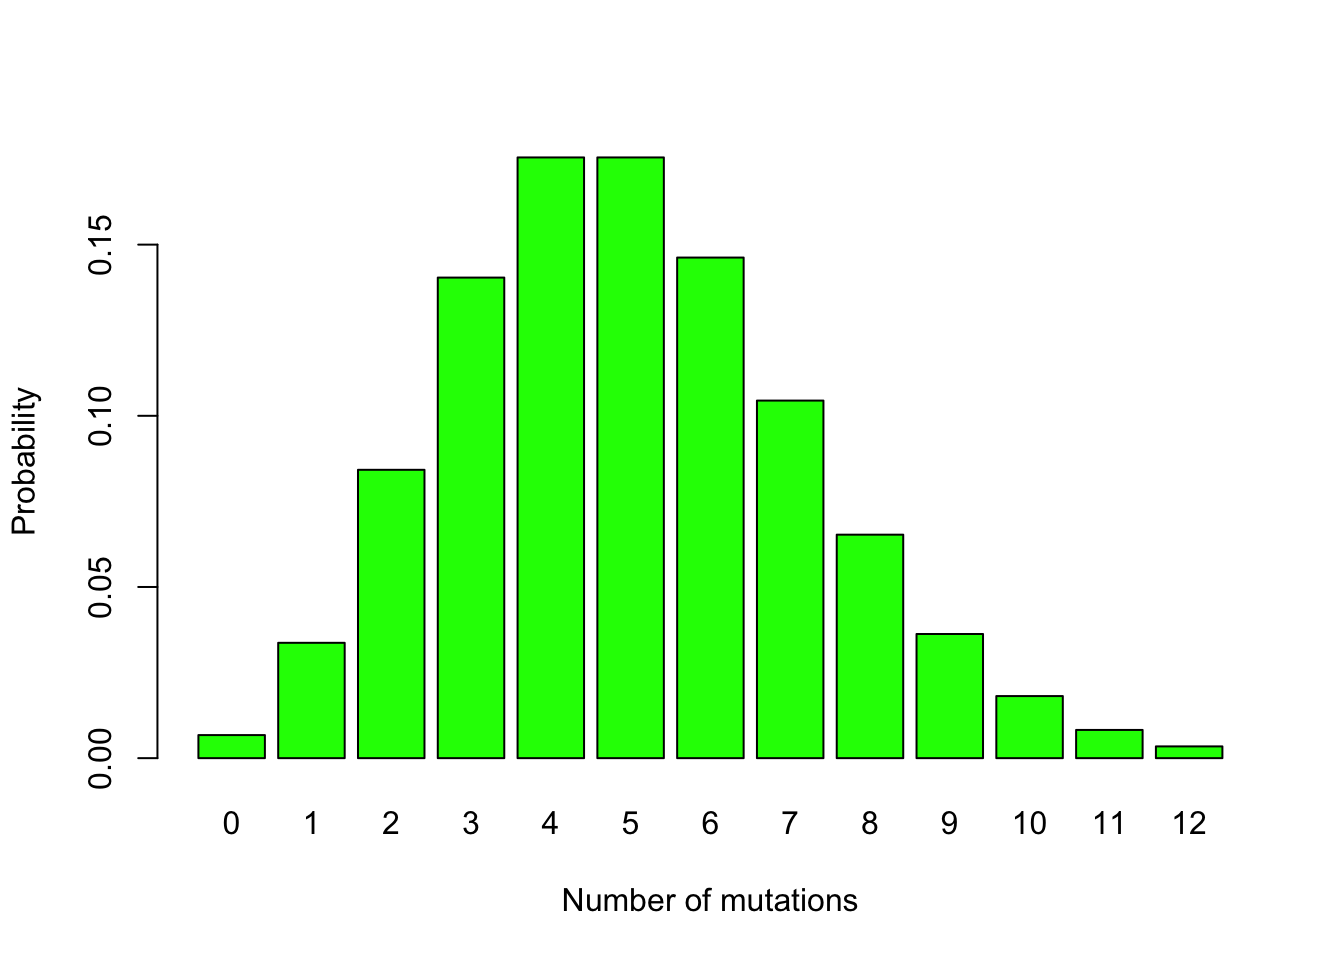
\includegraphics{Chapter4_files/figure-latex/unnamed-chunk-2-1.pdf}

We can use R's vectorized syntax to remove the vapply-loop and generate
the fairmix vector more efficiently.

\begin{Shaded}
\begin{Highlighting}[]
\NormalTok{means =}\StringTok{ }\KeywordTok{c}\NormalTok{(}\DecValTok{1}\NormalTok{, }\DecValTok{3}\NormalTok{)}
\NormalTok{sds   =}\StringTok{ }\KeywordTok{c}\NormalTok{(}\FloatTok{0.25}\NormalTok{, }\FloatTok{0.25}\NormalTok{)}
\NormalTok{values =}\StringTok{ }\KeywordTok{rnorm}\NormalTok{(}\KeywordTok{length}\NormalTok{(coinflips),}
          \DataTypeTok{mean =} \KeywordTok{ifelse}\NormalTok{(coinflips, means[}\DecValTok{1}\NormalTok{], means[}\DecValTok{2}\NormalTok{]),}
          \DataTypeTok{sd   =} \KeywordTok{ifelse}\NormalTok{(coinflips, sds[}\DecValTok{1}\NormalTok{],   sds[}\DecValTok{2}\NormalTok{]))}
\KeywordTok{ggplot}\NormalTok{(}\KeywordTok{tibble}\NormalTok{(}\DataTypeTok{value =}\NormalTok{ values), }\KeywordTok{aes}\NormalTok{(}\DataTypeTok{x =}\NormalTok{ value)) }\OperatorTok{+}
\StringTok{     }\KeywordTok{geom_histogram}\NormalTok{(}\DataTypeTok{fill =} \StringTok{"purple"}\NormalTok{, }\DataTypeTok{binwidth =} \FloatTok{0.1}\NormalTok{)}
\end{Highlighting}
\end{Shaded}

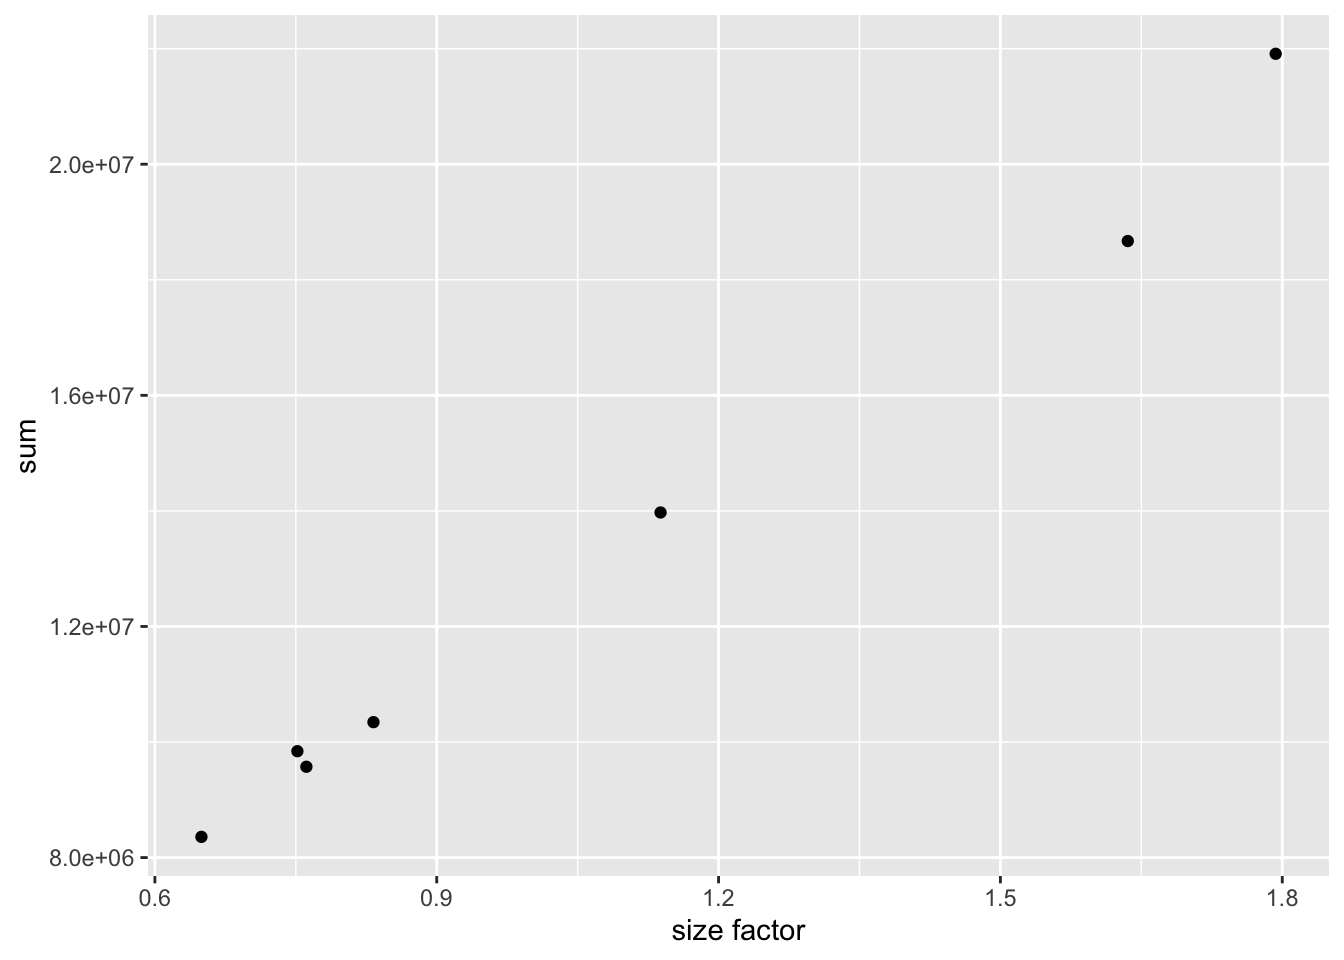
\includegraphics{Chapter4_files/figure-latex/unnamed-chunk-3-1.pdf}

What if we make one million coin flips and make a histogram with 500
bins

\begin{Shaded}
\begin{Highlighting}[]
\NormalTok{fair =}\StringTok{ }\KeywordTok{tibble}\NormalTok{(}
  \DataTypeTok{coinflips =}\NormalTok{ (}\KeywordTok{runif}\NormalTok{(}\FloatTok{1e6}\NormalTok{) }\OperatorTok{>}\StringTok{ }\FloatTok{0.5}\NormalTok{),}
  \DataTypeTok{values =} \KeywordTok{rnorm}\NormalTok{(}\KeywordTok{length}\NormalTok{(coinflips),}
               \DataTypeTok{mean =} \KeywordTok{ifelse}\NormalTok{(coinflips, means[}\DecValTok{1}\NormalTok{], means[}\DecValTok{2}\NormalTok{]),}
               \DataTypeTok{sd   =} \KeywordTok{ifelse}\NormalTok{(coinflips, sds[}\DecValTok{1}\NormalTok{],   sds[}\DecValTok{2}\NormalTok{])))}
\KeywordTok{ggplot}\NormalTok{(fair, }\KeywordTok{aes}\NormalTok{(}\DataTypeTok{x =}\NormalTok{ values)) }\OperatorTok{+}
\StringTok{     }\KeywordTok{geom_histogram}\NormalTok{(}\DataTypeTok{fill =} \StringTok{"purple"}\NormalTok{, }\DataTypeTok{bins =} \DecValTok{500}\NormalTok{)}
\end{Highlighting}
\end{Shaded}

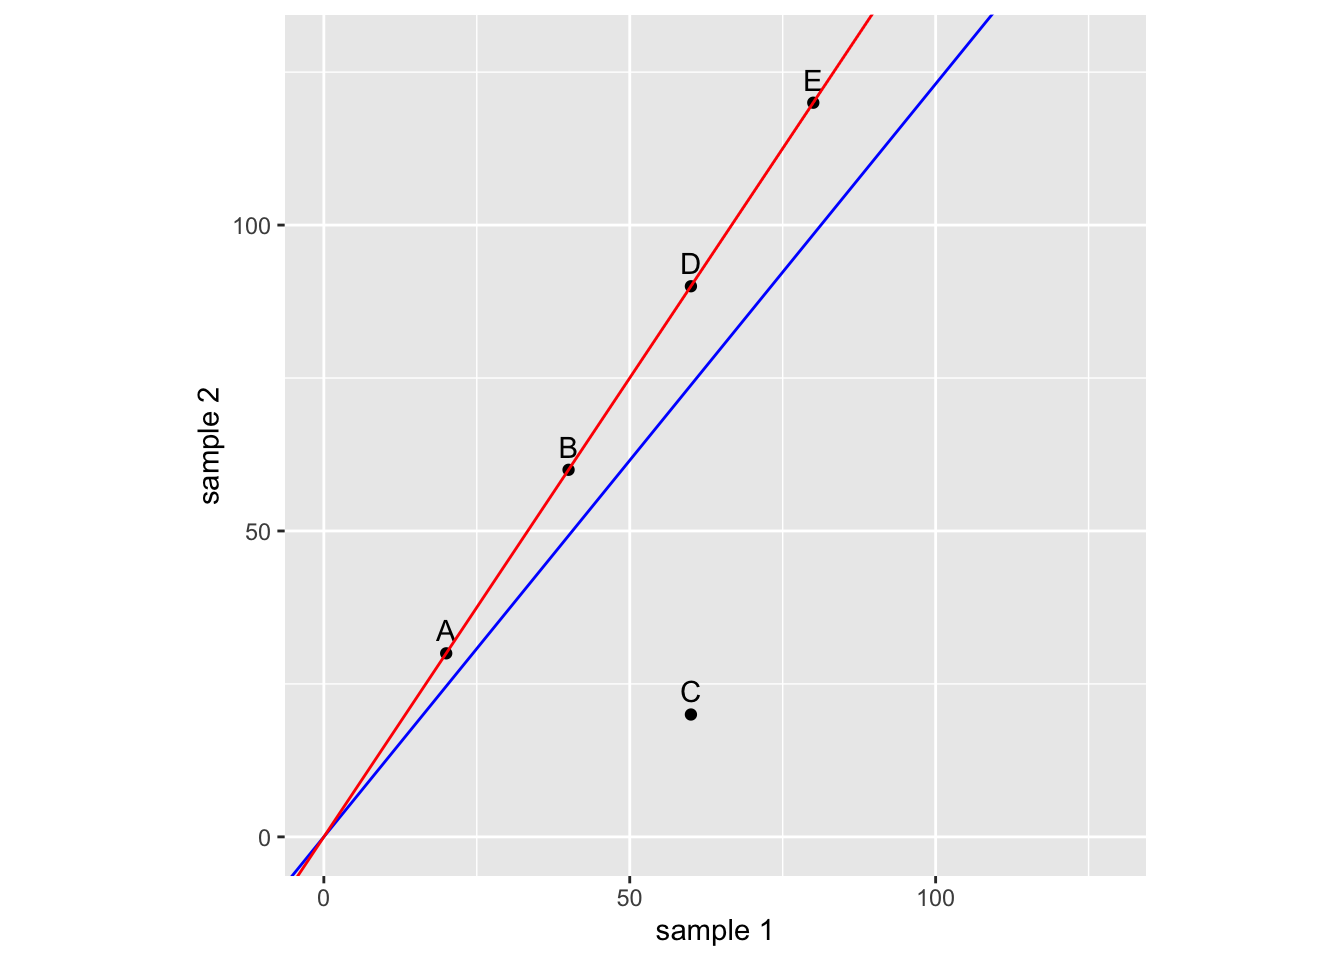
\includegraphics{Chapter4_files/figure-latex/unnamed-chunk-4-1.pdf} The
histogram gets nearer to a smooth curve called the density function
which offers a better approximation of the number of mixtures.

Compare the values of fair\$values for which coinflips is TRUE to
density function for a normal random variable.

\begin{Shaded}
\begin{Highlighting}[]
\KeywordTok{ggplot}\NormalTok{(dplyr}\OperatorTok{::}\KeywordTok{filter}\NormalTok{(fair, coinflips), }\KeywordTok{aes}\NormalTok{(}\DataTypeTok{x =}\NormalTok{ values)) }\OperatorTok{+}
\StringTok{   }\KeywordTok{geom_histogram}\NormalTok{(}\KeywordTok{aes}\NormalTok{(}\DataTypeTok{y =}\NormalTok{ ..density..), }\DataTypeTok{fill =} \StringTok{"purple"}\NormalTok{,}
                  \DataTypeTok{binwidth =} \FloatTok{0.01}\NormalTok{) }\OperatorTok{+}
\StringTok{   }\KeywordTok{stat_function}\NormalTok{(}\DataTypeTok{fun =}\NormalTok{ dnorm,}
          \DataTypeTok{args =} \KeywordTok{list}\NormalTok{(}\DataTypeTok{mean =}\NormalTok{ means[}\DecValTok{1}\NormalTok{], }\DataTypeTok{sd =}\NormalTok{ sds[}\DecValTok{1}\NormalTok{]), }\DataTypeTok{color =} \StringTok{"red"}\NormalTok{)}
\end{Highlighting}
\end{Shaded}

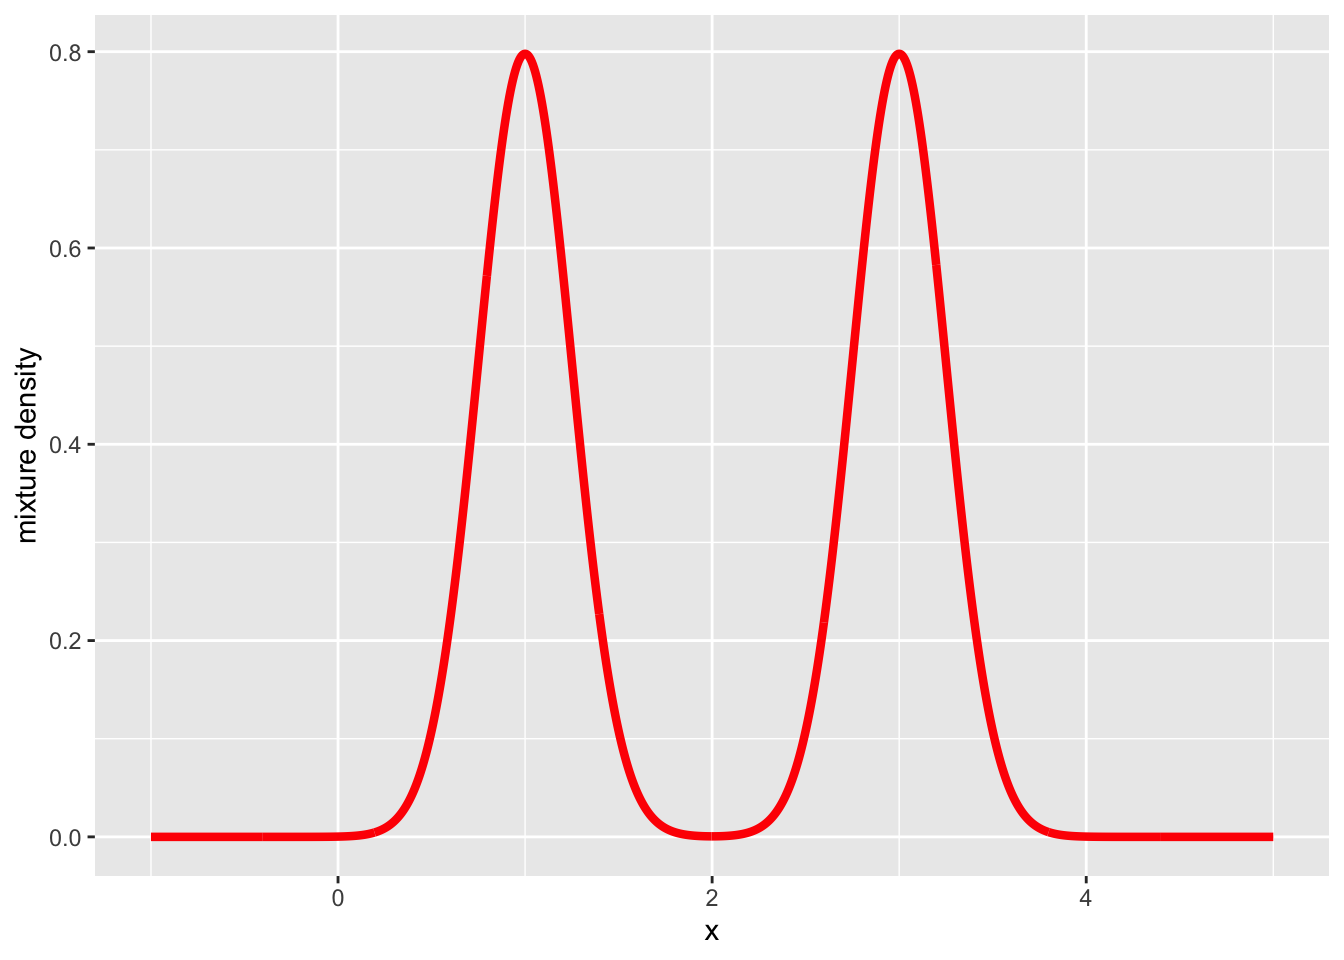
\includegraphics{Chapter4_files/figure-latex/unnamed-chunk-5-1.pdf}

Our distributions so far can be matematically represented as the sum of
the density distributions

We can use this concept to generate a graph for two component mixture
model with extremely visible distributions (using our previous mean and
standard deviations) and minimal overlap.

\begin{Shaded}
\begin{Highlighting}[]
\NormalTok{fairtheory =}\StringTok{ }\KeywordTok{tibble}\NormalTok{(}
  \DataTypeTok{x =} \KeywordTok{seq}\NormalTok{(}\OperatorTok{-}\DecValTok{1}\NormalTok{, }\DecValTok{5}\NormalTok{, }\DataTypeTok{length.out =} \DecValTok{1000}\NormalTok{),}
  \DataTypeTok{f =} \FloatTok{0.5} \OperatorTok{*}\StringTok{ }\KeywordTok{dnorm}\NormalTok{(x, }\DataTypeTok{mean =}\NormalTok{ means[}\DecValTok{1}\NormalTok{], }\DataTypeTok{sd =}\NormalTok{ sds[}\DecValTok{1}\NormalTok{]) }\OperatorTok{+}
\StringTok{      }\FloatTok{0.5} \OperatorTok{*}\StringTok{ }\KeywordTok{dnorm}\NormalTok{(x, }\DataTypeTok{mean =}\NormalTok{ means[}\DecValTok{2}\NormalTok{], }\DataTypeTok{sd =}\NormalTok{ sds[}\DecValTok{2}\NormalTok{]))}
\KeywordTok{ggplot}\NormalTok{(fairtheory, }\KeywordTok{aes}\NormalTok{(}\DataTypeTok{x =}\NormalTok{ x, }\DataTypeTok{y =}\NormalTok{ f)) }\OperatorTok{+}
\StringTok{  }\KeywordTok{geom_line}\NormalTok{(}\DataTypeTok{color =} \StringTok{"red"}\NormalTok{, }\DataTypeTok{size =} \FloatTok{1.5}\NormalTok{) }\OperatorTok{+}\StringTok{ }\KeywordTok{ylab}\NormalTok{(}\StringTok{"mixture density"}\NormalTok{)}
\end{Highlighting}
\end{Shaded}

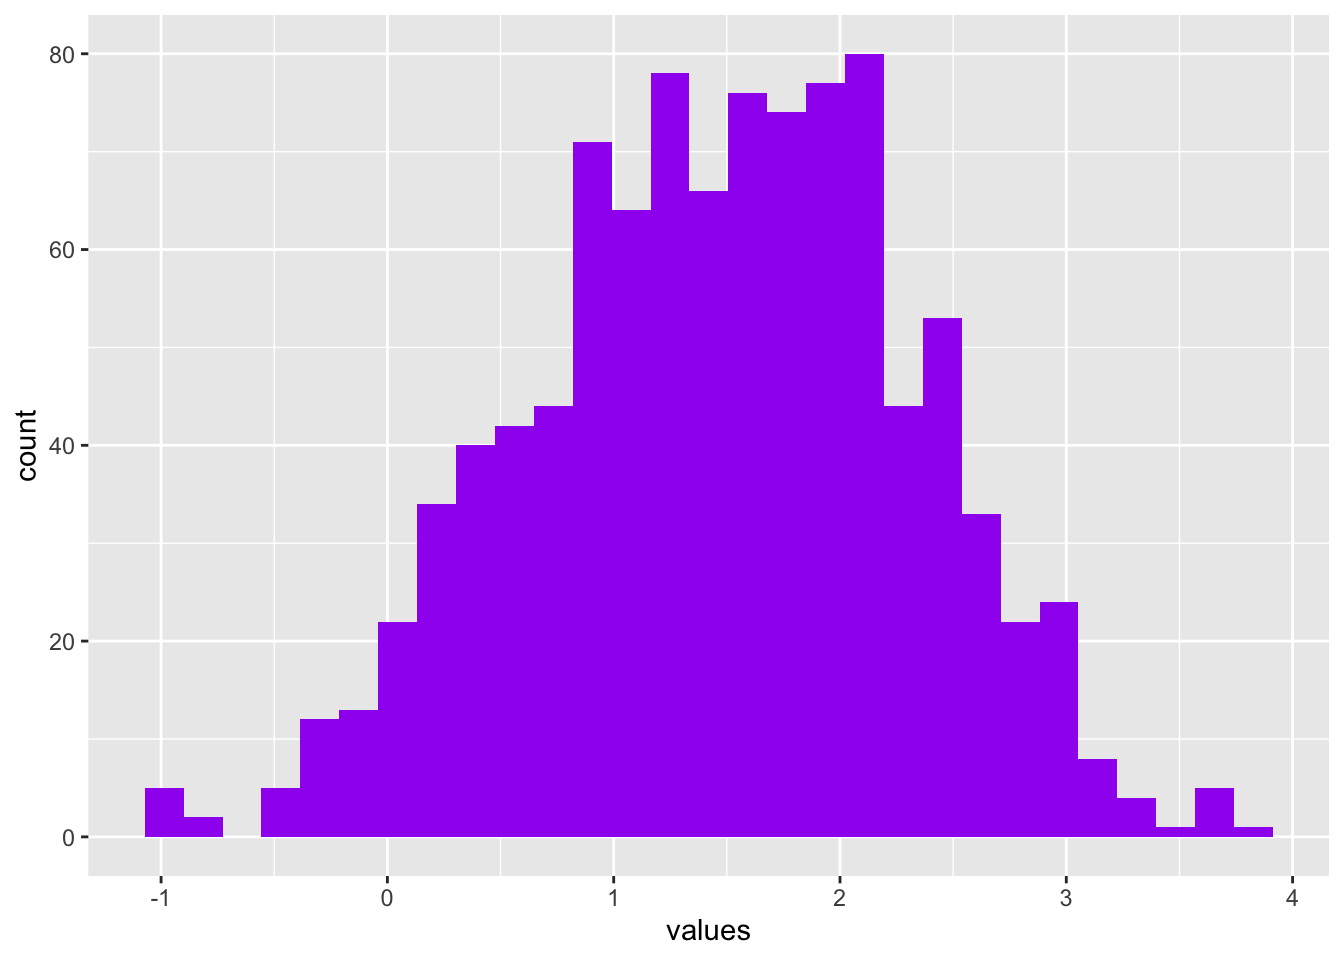
\includegraphics{Chapter4_files/figure-latex/unnamed-chunk-6-1.pdf}

What if we had a figure generated by the code chunk below (means= 1 and
2; std= sqrt(.5) and sqrt(.5) ) without afore knowledge of the code.
That is we form a hard-to -esolve distribution as the means of the
individual distributions gets closer and the variance increases.

\begin{Shaded}
\begin{Highlighting}[]
\KeywordTok{set.seed}\NormalTok{(}\DecValTok{1234}\NormalTok{)}
\NormalTok{mystery =}\StringTok{ }\KeywordTok{tibble}\NormalTok{(}
  \DataTypeTok{coinflips =}\NormalTok{ (}\KeywordTok{runif}\NormalTok{(}\FloatTok{1e3}\NormalTok{) }\OperatorTok{>}\StringTok{ }\FloatTok{0.5}\NormalTok{),}
  \DataTypeTok{values =} \KeywordTok{rnorm}\NormalTok{(}\KeywordTok{length}\NormalTok{(coinflips),}
               \DataTypeTok{mean =} \KeywordTok{ifelse}\NormalTok{(coinflips, }\DecValTok{1}\NormalTok{, }\DecValTok{2}\NormalTok{),}
               \DataTypeTok{sd   =} \KeywordTok{ifelse}\NormalTok{(coinflips, }\KeywordTok{sqrt}\NormalTok{(.}\DecValTok{5}\NormalTok{), }\KeywordTok{sqrt}\NormalTok{(.}\DecValTok{5}\NormalTok{))))}
\NormalTok{br2 =}\StringTok{ }\KeywordTok{with}\NormalTok{(mystery, }\KeywordTok{seq}\NormalTok{(}\KeywordTok{min}\NormalTok{(values), }\KeywordTok{max}\NormalTok{(values), }\DataTypeTok{length.out =} \DecValTok{30}\NormalTok{))}
\KeywordTok{ggplot}\NormalTok{(mystery, }\KeywordTok{aes}\NormalTok{(}\DataTypeTok{x =}\NormalTok{ values)) }\OperatorTok{+}
\KeywordTok{geom_histogram}\NormalTok{(}\DataTypeTok{fill =} \StringTok{"purple"}\NormalTok{, }\DataTypeTok{breaks =}\NormalTok{ br2)}
\end{Highlighting}
\end{Shaded}

\includegraphics{Chapter4_files/figure-latex/unnamed-chunk-7-1.pdf}

\begin{Shaded}
\begin{Highlighting}[]
\KeywordTok{head}\NormalTok{(mystery, }\DecValTok{3}\NormalTok{)}
\end{Highlighting}
\end{Shaded}

\begin{verbatim}
## # A tibble: 3 x 2
##   coinflips values
##   <lgl>      <dbl>
## 1 FALSE      2.70 
## 2 TRUE       0.134
## 3 TRUE       1.50
\end{verbatim}

\begin{Shaded}
\begin{Highlighting}[]
\NormalTok{br =}\StringTok{ }\KeywordTok{with}\NormalTok{(mystery, }\KeywordTok{seq}\NormalTok{(}\KeywordTok{min}\NormalTok{(values), }\KeywordTok{max}\NormalTok{(values), }\DataTypeTok{length.out =} \DecValTok{30}\NormalTok{))}
\KeywordTok{ggplot}\NormalTok{(mystery, }\KeywordTok{aes}\NormalTok{(}\DataTypeTok{x =}\NormalTok{ values)) }\OperatorTok{+}
\StringTok{  }\KeywordTok{geom_histogram}\NormalTok{(}\DataTypeTok{data =}\NormalTok{ dplyr}\OperatorTok{::}\KeywordTok{filter}\NormalTok{(mystery, coinflips),}
     \DataTypeTok{fill =} \StringTok{"red"}\NormalTok{, }\DataTypeTok{alpha =} \FloatTok{0.2}\NormalTok{, }\DataTypeTok{breaks =}\NormalTok{ br) }\OperatorTok{+}
\StringTok{  }\KeywordTok{geom_histogram}\NormalTok{(}\DataTypeTok{data =}\NormalTok{ dplyr}\OperatorTok{::}\KeywordTok{filter}\NormalTok{(mystery, }\OperatorTok{!}\NormalTok{coinflips),}
     \DataTypeTok{fill =} \StringTok{"darkblue"}\NormalTok{, }\DataTypeTok{alpha =} \FloatTok{0.2}\NormalTok{, }\DataTypeTok{breaks =}\NormalTok{ br) }
\end{Highlighting}
\end{Shaded}

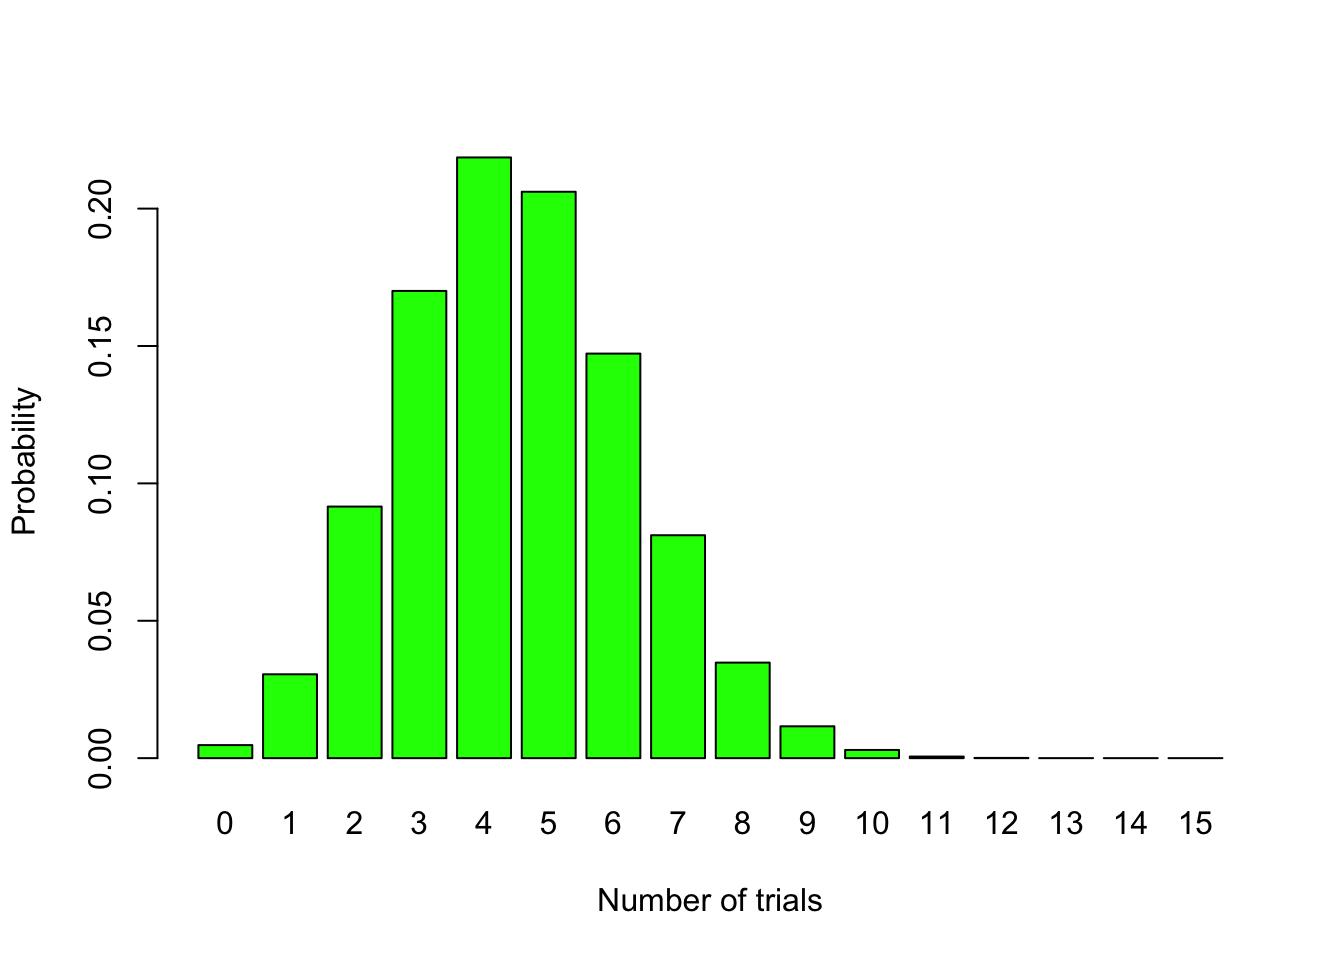
\includegraphics{Chapter4_files/figure-latex/unnamed-chunk-8-1.pdf}

\begin{Shaded}
\begin{Highlighting}[]
\CommentTok{#This code separtes the distributions and treats overlaps as belonging to separate groups. This is evident from the heights of the bars.}
\end{Highlighting}
\end{Shaded}

We can now plot all the ``mystery'' graphs in layers over each other

\begin{Shaded}
\begin{Highlighting}[]
\KeywordTok{ggplot}\NormalTok{(mystery, }\KeywordTok{aes}\NormalTok{(}\DataTypeTok{x =}\NormalTok{ values, }\DataTypeTok{fill =}\NormalTok{ coinflips)) }\OperatorTok{+}
\StringTok{  }\KeywordTok{geom_histogram}\NormalTok{(}\DataTypeTok{data =}\NormalTok{ dplyr}\OperatorTok{::}\KeywordTok{filter}\NormalTok{(mystery, coinflips),}
     \DataTypeTok{fill =} \StringTok{"red"}\NormalTok{, }\DataTypeTok{alpha =} \FloatTok{0.2}\NormalTok{, }\DataTypeTok{breaks =}\NormalTok{ br) }\OperatorTok{+}
\StringTok{  }\KeywordTok{geom_histogram}\NormalTok{(}\DataTypeTok{data =}\NormalTok{ dplyr}\OperatorTok{::}\KeywordTok{filter}\NormalTok{(mystery, }\OperatorTok{!}\NormalTok{coinflips),}
     \DataTypeTok{fill =} \StringTok{"darkblue"}\NormalTok{, }\DataTypeTok{alpha =} \FloatTok{0.2}\NormalTok{, }\DataTypeTok{breaks =}\NormalTok{ br) }\OperatorTok{+}
\StringTok{  }\KeywordTok{geom_histogram}\NormalTok{(}\DataTypeTok{fill =} \StringTok{"purple"}\NormalTok{, }\DataTypeTok{breaks =}\NormalTok{ br, }\DataTypeTok{alpha =} \FloatTok{0.2}\NormalTok{)}
\end{Highlighting}
\end{Shaded}

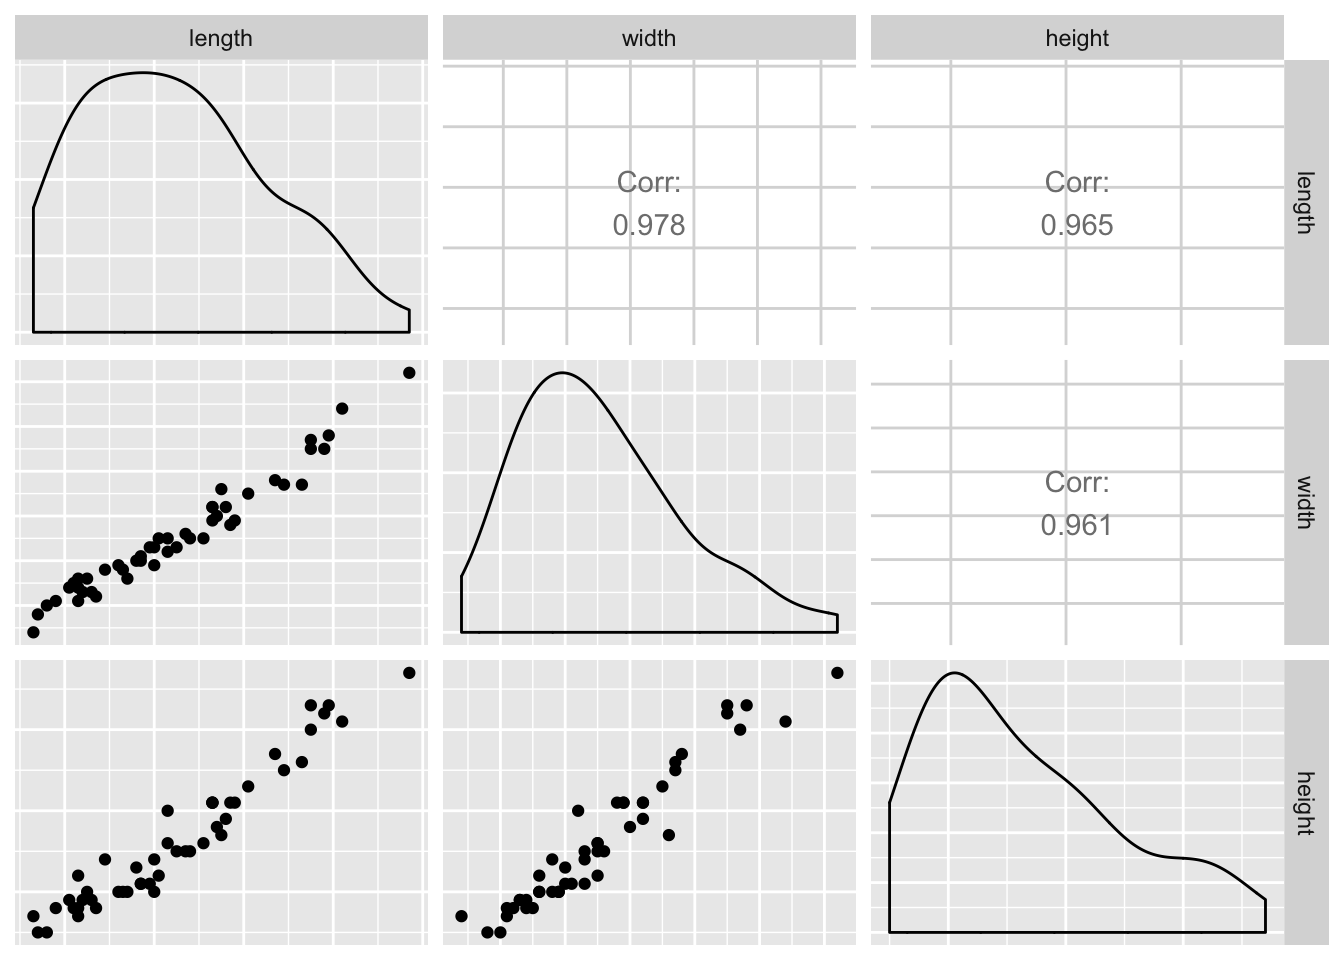
\includegraphics{Chapter4_files/figure-latex/unnamed-chunk-9-1.pdf}

\hypertarget{the-expectation-maximization-em-algorithm}{%
\subsubsection{The Expectation-Maximization (EM)
Algorithm}\label{the-expectation-maximization-em-algorithm}}

The EM algorithm is used to infer the value of hidden groupings. It does
so by; alternating between:\\
- Pretending to know the probability that each observation belongs to a
component (and estimating the distribution paramaters of these
components)\\
- Pretending to know the distribution parameters of each component (and
estimating the probability that each observation belongs to a given
component)

probHead = c(0.125, 0.25) for (pi in c(1/8, 1/4)) \{ whCoin = sample(2,
100, replace = TRUE, prob = c(pi, 1-pi)) K = rbinom(length(whCoin), size
= 2, prob = probHead{[}whCoin{]}) print(table(K)) \}

For example a variable Y is measured on a series of objects that come
from two groups (however we do not know which group each object belongs
to). The goal is to estimate the parameters that make the data Y This
can be done by;\\
- Augmenting the data with a latent (unobserved/hidden) variable, U.this
resuls in a bivariate distribution because we are looking at the
distribution of ``couples'' (Y,U) - Adopting the Maximum Likelihood
approach to find the values of U and the unknown parameters of
underlying densities.

Scenario 1 Suppose we have two unfair coins, whose probabilities of
heads are p1=0.125 and p2=0.25. With probability pi we pick coin 1, with
probability = 1−pi, coin 2. We then toss that coin twice and record the
number of heads K. a) Simulate 100 instances of this procedure, with
pi=1/8, and compute the contingency table of K. b) Do the same with
pi=1/4. c) Can the afore mentioned parameters parameters from the
contingency table?

Solution

\begin{Shaded}
\begin{Highlighting}[]
\NormalTok{probHead =}\StringTok{ }\KeywordTok{c}\NormalTok{(}\FloatTok{0.125}\NormalTok{, }\FloatTok{0.25}\NormalTok{)}
\KeywordTok{set.seed}\NormalTok{(}\DecValTok{1234}\NormalTok{)}
\ControlFlowTok{for}\NormalTok{ (pi }\ControlFlowTok{in} \KeywordTok{c}\NormalTok{(}\DecValTok{1}\OperatorTok{/}\DecValTok{8}\NormalTok{, }\DecValTok{1}\OperatorTok{/}\DecValTok{4}\NormalTok{)) \{}
\NormalTok{  whCoin =}\StringTok{ }\KeywordTok{sample}\NormalTok{(}\DecValTok{2}\NormalTok{, }\DecValTok{100}\NormalTok{, }\DataTypeTok{replace =} \OtherTok{TRUE}\NormalTok{, }\DataTypeTok{prob =} \KeywordTok{c}\NormalTok{(pi, }\DecValTok{1}\OperatorTok{-}\NormalTok{pi))}
\NormalTok{  K =}\StringTok{ }\KeywordTok{rbinom}\NormalTok{(}\KeywordTok{length}\NormalTok{(whCoin), }\DataTypeTok{size =} \DecValTok{2}\NormalTok{, }\DataTypeTok{prob =}\NormalTok{ probHead[whCoin])}
  \KeywordTok{print}\NormalTok{(}\KeywordTok{table}\NormalTok{(K))}
\NormalTok{\}}
\end{Highlighting}
\end{Shaded}

\begin{verbatim}
## K
##  0  1  2 
## 55 33 12 
## K
##  0  1  2 
## 60 29 11
\end{verbatim}

The parameter are difficult to estimate due to the numerous degrees of
freedom.

Scenario 2 Estimating the parameters of a mixture of two normals with
mean parameters unkown and standard deviation equal to 1.

\begin{Shaded}
\begin{Highlighting}[]
\CommentTok{# generate  model with R using the labels "u"}
\CommentTok{#randomly sample 1 or 2, 100 times, with replacement}
\NormalTok{mus =}\StringTok{ }\KeywordTok{c}\NormalTok{(}\OperatorTok{-}\FloatTok{0.5}\NormalTok{, }\FloatTok{1.5}\NormalTok{)}
\KeywordTok{set.seed}\NormalTok{(}\DecValTok{1234}\NormalTok{)}
\NormalTok{u =}\StringTok{ }\KeywordTok{sample}\NormalTok{(}\DecValTok{2}\NormalTok{, }\DecValTok{100}\NormalTok{, }\DataTypeTok{replace =} \OtherTok{TRUE}\NormalTok{)}
\CommentTok{#create a random normal distribution of 100 numbers with mean equal to -0.5(1) or 1.5(2)}
\NormalTok{y =}\StringTok{ }\KeywordTok{rnorm}\NormalTok{(}\KeywordTok{length}\NormalTok{(u), }\DataTypeTok{mean =}\NormalTok{ mus[u])}
\NormalTok{duy =}\StringTok{ }\KeywordTok{tibble}\NormalTok{(u, y)}
\KeywordTok{head}\NormalTok{(duy)}
\end{Highlighting}
\end{Shaded}

\begin{verbatim}
## # A tibble: 6 x 2
##       u      y
##   <int>  <dbl>
## 1     2 -0.306
## 2     2  0.918
## 3     2  0.391
## 4     2  0.485
## 5     1 -0.662
## 6     2  2.06
\end{verbatim}

Since we know the labels ``u'', we can estimate the means by using
seperate ML equations for each group.

\begin{Shaded}
\begin{Highlighting}[]
\NormalTok{duy }\OperatorTok\StringTok{ }\KeywordTok{group_by}\NormalTok{(u) }\OperatorTok\StringTok{ }\KeywordTok{summarise}\NormalTok{(}\KeywordTok{mean}\NormalTok{(y))}
\end{Highlighting}
\end{Shaded}

\begin{verbatim}
## # A tibble: 2 x 2
##       u `mean(y)`
##   <int>     <dbl>
## 1     1    -0.479
## 2     2     1.62
\end{verbatim}

\begin{Shaded}
\begin{Highlighting}[]
\NormalTok{EMtest <-}\StringTok{ }\KeywordTok{Mclust}\NormalTok{(duy}\OperatorTok{$}\NormalTok{y, }\DataTypeTok{nclass=}\DecValTok{2}\NormalTok{)}
\NormalTok{EMtest}\OperatorTok{$}\NormalTok{n}
\end{Highlighting}
\end{Shaded}

\begin{verbatim}
## [1] 100
\end{verbatim}

\begin{Shaded}
\begin{Highlighting}[]
\NormalTok{EMtest}\OperatorTok{$}\NormalTok{df}
\end{Highlighting}
\end{Shaded}

\begin{verbatim}
## [1] 2
\end{verbatim}

\begin{Shaded}
\begin{Highlighting}[]
\NormalTok{EMtest}\OperatorTok{$}\NormalTok{BIC}
\end{Highlighting}
\end{Shaded}

\begin{verbatim}
## Bayesian Information Criterion (BIC): 
##           E         V
## 1 -360.6557 -360.6557
## 2 -367.9925 -367.3822
## 3 -371.8851 -382.3664
## 4 -375.8227 -386.7824
## 5 -383.3537 -398.3807
## 6 -388.2105 -403.3627
## 7 -397.4478 -414.0851
## 8 -406.6570 -427.8954
## 9 -415.9232 -436.2490
## 
## Top 3 models based on the BIC criterion: 
##       E,1       V,1       V,2 
## -360.6557 -360.6557 -367.3822
\end{verbatim}

\begin{Shaded}
\begin{Highlighting}[]
\NormalTok{EMtest}\OperatorTok{$}\NormalTok{classification}
\end{Highlighting}
\end{Shaded}

\begin{verbatim}
##   [1] 1 1 1 1 1 1 1 1 1 1 1 1 1 1 1 1 1 1 1 1 1 1 1 1 1 1 1 1 1 1 1 1 1 1 1
##  [36] 1 1 1 1 1 1 1 1 1 1 1 1 1 1 1 1 1 1 1 1 1 1 1 1 1 1 1 1 1 1 1 1 1 1 1
##  [71] 1 1 1 1 1 1 1 1 1 1 1 1 1 1 1 1 1 1 1 1 1 1 1 1 1 1 1 1 1 1
\end{verbatim}

\begin{Shaded}
\begin{Highlighting}[]
\KeywordTok{head}\NormalTok{(duy}\OperatorTok{$}\NormalTok{u,}\DecValTok{20}\NormalTok{)}
\end{Highlighting}
\end{Shaded}

\begin{verbatim}
##  [1] 2 2 2 2 1 2 1 1 1 2 2 2 2 1 2 2 2 1 2 2
\end{verbatim}

\begin{Shaded}
\begin{Highlighting}[]
\NormalTok{gm <-}\StringTok{ }\KeywordTok{normalmixEM}\NormalTok{(duy}\OperatorTok{$}\NormalTok{y, }\DataTypeTok{k=}\DecValTok{2}\NormalTok{, }\DataTypeTok{lambda=}\KeywordTok{c}\NormalTok{(}\FloatTok{0.5}\NormalTok{,}\FloatTok{0.5}\NormalTok{), }\DataTypeTok{mu=}\KeywordTok{c}\NormalTok{(}\OperatorTok{-}\FloatTok{0.01}\NormalTok{,}\FloatTok{0.01}\NormalTok{), }\DataTypeTok{sigma=}\KeywordTok{c}\NormalTok{(}\DecValTok{1}\NormalTok{,}\DecValTok{1}\NormalTok{))}
\end{Highlighting}
\end{Shaded}

\begin{verbatim}
## number of iterations= 563
\end{verbatim}

\begin{Shaded}
\begin{Highlighting}[]
\NormalTok{gm}\OperatorTok{$}\NormalTok{lambda}
\end{Highlighting}
\end{Shaded}

\begin{verbatim}
## [1] 0.09610953 0.90389047
\end{verbatim}

\begin{Shaded}
\begin{Highlighting}[]
\NormalTok{gm}\OperatorTok{$}\NormalTok{mu}
\end{Highlighting}
\end{Shaded}

\begin{verbatim}
## [1] -1.6326458  0.9920098
\end{verbatim}

\begin{Shaded}
\begin{Highlighting}[]
\NormalTok{gm}\OperatorTok{$}\NormalTok{sigma}
\end{Highlighting}
\end{Shaded}

\begin{verbatim}
## [1] 0.3038369 1.2265384
\end{verbatim}

\begin{Shaded}
\begin{Highlighting}[]
\NormalTok{gm}\OperatorTok{$}\NormalTok{loglik}
\end{Highlighting}
\end{Shaded}

\begin{verbatim}
## [1] -172.1765
\end{verbatim}

\hypertarget{models-for-zero-inflated-data}{%
\subsection{Models for zero inflated
data}\label{models-for-zero-inflated-data}}

Ecological and molecular data often come in the form of counts. Such as
the count data in RNA seq. Such data can often be seen as a mixture of
two scenarios: a. If gene is not expressed the count is zero b. It gene
is expressed the number of transcripts in different individuals may
differ

The R packages pscl and zicounts provide many examples and functions for
working with zero inflated counts.

Demonstration with chromatin immunoprecipitation (ChIP) data

\begin{Shaded}
\begin{Highlighting}[]
\KeywordTok{constructBins}\NormalTok{(}\DataTypeTok{infile =} \KeywordTok{system.file}\NormalTok{(}\KeywordTok{file.path}\NormalTok{(}\StringTok{"extdata"}\NormalTok{, }\StringTok{"wgEncodeSydhTfbsGm12878Stat1StdAlnRep1_chr22_sorted.bam"}\NormalTok{), }\DataTypeTok{package=}\StringTok{"mosaicsExample"}\NormalTok{),}
    \DataTypeTok{fileFormat =} \StringTok{"bam"}\NormalTok{, }\DataTypeTok{outfileLoc =} \KeywordTok{here}\NormalTok{(}\StringTok{"Book"}\NormalTok{, }\StringTok{"data"}\NormalTok{),}
    \DataTypeTok{byChr =} \OtherTok{FALSE}\NormalTok{, }\DataTypeTok{useChrfile =} \OtherTok{FALSE}\NormalTok{, }\DataTypeTok{chrfile =} \OtherTok{NULL}\NormalTok{, }\DataTypeTok{excludeChr =} \OtherTok{NULL}\NormalTok{,}
    \DataTypeTok{PET =} \OtherTok{FALSE}\NormalTok{, }\DataTypeTok{fragLen =} \DecValTok{200}\NormalTok{, }\DataTypeTok{binSize =} \DecValTok{200}\NormalTok{, }\DataTypeTok{capping =} \DecValTok{0}\NormalTok{)}
\end{Highlighting}
\end{Shaded}

\begin{verbatim}
## ------------------------------------------------------------
## Info: setting summary
## ------------------------------------------------------------
## Name of aligned read file: /Library/Frameworks/R.framework/Versions/3.6/Resources/library/mosaicsExample/extdata/wgEncodeSydhTfbsGm12878Stat1StdAlnRep1_chr22_sorted.bam 
## Aligned read file format: BAM 
## Directory of processed bin-level files: /Users/abdul-rahmanbukari/Documents/BIOSTATS/Book/data 
## Construct bin-level files by chromosome? N 
## Is file for chromosome info provided? N 
## Data type: Single-end tag (SET)
## Average fragment length: 200 
## Bin size: 200 
## ------------------------------------------------------------
\end{verbatim}

\begin{verbatim}
## Use the provided BAM index file.
\end{verbatim}

\begin{verbatim}
## Chromosome information is extracted from the BAM file.
\end{verbatim}

\begin{verbatim}
## Info: reading the aligned read file and processing it into bin-level files...
\end{verbatim}

\begin{verbatim}
## Info: done!
\end{verbatim}

\begin{verbatim}
## ------------------------------------------------------------
## Info: processing summary
## ------------------------------------------------------------
## Directory of processed bin-level files: /Users/abdul-rahmanbukari/Documents/BIOSTATS/Book/data 
## Processed bin-level file: wgEncodeSydhTfbsGm12878Stat1StdAlnRep1_chr22_sorted.bam_fragL200_bin200.txt
## Sequencing depth: 231822 
## ------------------------------------------------------------
\end{verbatim}

\begin{Shaded}
\begin{Highlighting}[]
\KeywordTok{constructBins}\NormalTok{(}\DataTypeTok{infile =} \KeywordTok{system.file}\NormalTok{(}\KeywordTok{file.path}\NormalTok{(}\StringTok{"extdata"}\NormalTok{, }\StringTok{"wgEncodeSydhTfbsGm12878InputStdAlnRep1_chr22_sorted.bam"}\NormalTok{), }\DataTypeTok{package=}\StringTok{"mosaicsExample"}\NormalTok{),}
    \DataTypeTok{fileFormat =} \StringTok{"bam"}\NormalTok{, }\DataTypeTok{outfileLoc =} \KeywordTok{here}\NormalTok{(}\StringTok{"Book"}\NormalTok{, }\StringTok{"data"}\NormalTok{),}
    \DataTypeTok{byChr =} \OtherTok{FALSE}\NormalTok{, }\DataTypeTok{useChrfile =} \OtherTok{FALSE}\NormalTok{, }\DataTypeTok{chrfile =} \OtherTok{NULL}\NormalTok{, }\DataTypeTok{excludeChr =} \OtherTok{NULL}\NormalTok{,}
    \DataTypeTok{PET =} \OtherTok{FALSE}\NormalTok{, }\DataTypeTok{fragLen =} \DecValTok{200}\NormalTok{, }\DataTypeTok{binSize =} \DecValTok{200}\NormalTok{, }\DataTypeTok{capping =} \DecValTok{0}\NormalTok{)}
\end{Highlighting}
\end{Shaded}

\begin{verbatim}
## ------------------------------------------------------------
## Info: setting summary
## ------------------------------------------------------------
## Name of aligned read file: /Library/Frameworks/R.framework/Versions/3.6/Resources/library/mosaicsExample/extdata/wgEncodeSydhTfbsGm12878InputStdAlnRep1_chr22_sorted.bam 
## Aligned read file format: BAM 
## Directory of processed bin-level files: /Users/abdul-rahmanbukari/Documents/BIOSTATS/Book/data 
## Construct bin-level files by chromosome? N 
## Is file for chromosome info provided? N 
## Data type: Single-end tag (SET)
## Average fragment length: 200 
## Bin size: 200 
## ------------------------------------------------------------
\end{verbatim}

\begin{verbatim}
## Use the provided BAM index file.
\end{verbatim}

\begin{verbatim}
## Chromosome information is extracted from the BAM file.
\end{verbatim}

\begin{verbatim}
## Info: reading the aligned read file and processing it into bin-level files...
\end{verbatim}

\begin{verbatim}
## Info: done!
\end{verbatim}

\begin{verbatim}
## ------------------------------------------------------------
## Info: processing summary
## ------------------------------------------------------------
## Directory of processed bin-level files: /Users/abdul-rahmanbukari/Documents/BIOSTATS/Book/data 
## Processed bin-level file: wgEncodeSydhTfbsGm12878InputStdAlnRep1_chr22_sorted.bam_fragL200_bin200.txt
## Sequencing depth: 182605 
## ------------------------------------------------------------
\end{verbatim}

\begin{Shaded}
\begin{Highlighting}[]
\NormalTok{datafiles =}\StringTok{ }\KeywordTok{c}\NormalTok{(}\KeywordTok{here}\NormalTok{(}\StringTok{"Book"}\NormalTok{,}\StringTok{"data"}\NormalTok{,}\StringTok{"wgEncodeSydhTfbsGm12878Stat1StdAlnRep1_chr22_sorted.bam_fragL200_bin200.txt"}\NormalTok{), }\KeywordTok{here}\NormalTok{(}\StringTok{"Book"}\NormalTok{, }\StringTok{"data"}\NormalTok{,}\StringTok{"wgEncodeSydhTfbsGm12878InputStdAlnRep1_chr22_sorted.bam_fragL200_bin200.txt"}\NormalTok{))}
\NormalTok{binTFBS =}\StringTok{ }\KeywordTok{readBins}\NormalTok{(}\DataTypeTok{type =} \KeywordTok{c}\NormalTok{(}\StringTok{"chip"}\NormalTok{,}\StringTok{"input"}\NormalTok{), }\DataTypeTok{fileName =}\NormalTok{ datafiles)}
\end{Highlighting}
\end{Shaded}

\begin{verbatim}
## Info: reading and preprocessing bin-level data...
\end{verbatim}

\begin{verbatim}
## Info: data contains only one chromosome.
\end{verbatim}

\begin{verbatim}
## Info: done!
\end{verbatim}

\begin{Shaded}
\begin{Highlighting}[]
\NormalTok{binTFBS}
\end{Highlighting}
\end{Shaded}

\begin{verbatim}
## Summary: bin-level data (class: BinData)
## ----------------------------------------
## - # of chromosomes in the data: 1
## - total effective tag counts: 462479
##   (sum of ChIP tag counts of all bins)
## - control sample is incorporated
## - mappability score is NOT incorporated
## - GC content score is NOT incorporated
## - uni-reads are assumed
## ----------------------------------------
\end{verbatim}

\begin{Shaded}
\begin{Highlighting}[]
\NormalTok{bincts =}\StringTok{ }\KeywordTok{print}\NormalTok{(binTFBS)}
\KeywordTok{ggplot}\NormalTok{(bincts, }\KeywordTok{aes}\NormalTok{(}\DataTypeTok{x =}\NormalTok{ tagCount)) }\OperatorTok{+}
\StringTok{  }\KeywordTok{geom_histogram}\NormalTok{(}\DataTypeTok{binwidth =} \DecValTok{1}\NormalTok{, }\DataTypeTok{fill =} \StringTok{"forestgreen"}\NormalTok{)}
\end{Highlighting}
\end{Shaded}

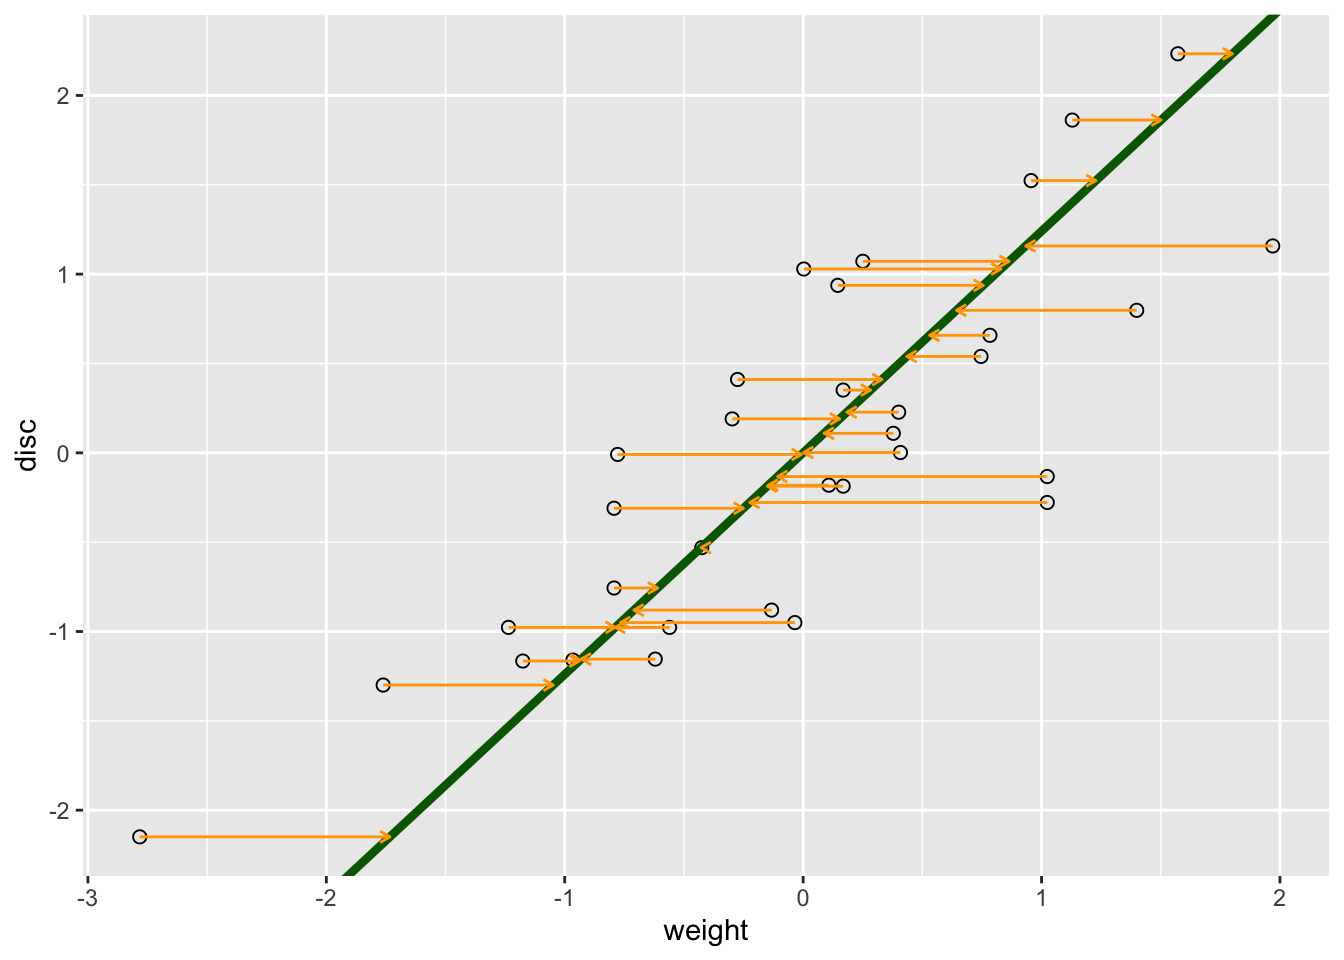
\includegraphics{Chapter4_files/figure-latex/unnamed-chunk-16-1.pdf}

It can be observed that there are many zeros, although from this plot it
is not immediately obvious whether the number of zeros is really
extraordinary, given the frequencies of the other small numbers Let's
edo the histogram of the counts using a logarithm base 10 scale on the y
and estimate π0, the proportion of bins with zero counts.

\begin{Shaded}
\begin{Highlighting}[]
\KeywordTok{ggplot}\NormalTok{(bincts, }\KeywordTok{aes}\NormalTok{(}\DataTypeTok{x =}\NormalTok{ tagCount)) }\OperatorTok{+}\StringTok{ }\KeywordTok{scale_y_log10}\NormalTok{() }\OperatorTok{+}
\StringTok{   }\KeywordTok{geom_histogram}\NormalTok{(}\DataTypeTok{binwidth =} \DecValTok{1}\NormalTok{, }\DataTypeTok{fill =} \StringTok{"forestgreen"}\NormalTok{)}
\end{Highlighting}
\end{Shaded}

\begin{verbatim}
## Warning: Transformation introduced infinite values in continuous y-axis
\end{verbatim}

\begin{verbatim}
## Warning: Removed 17 rows containing missing values (geom_bar).
\end{verbatim}

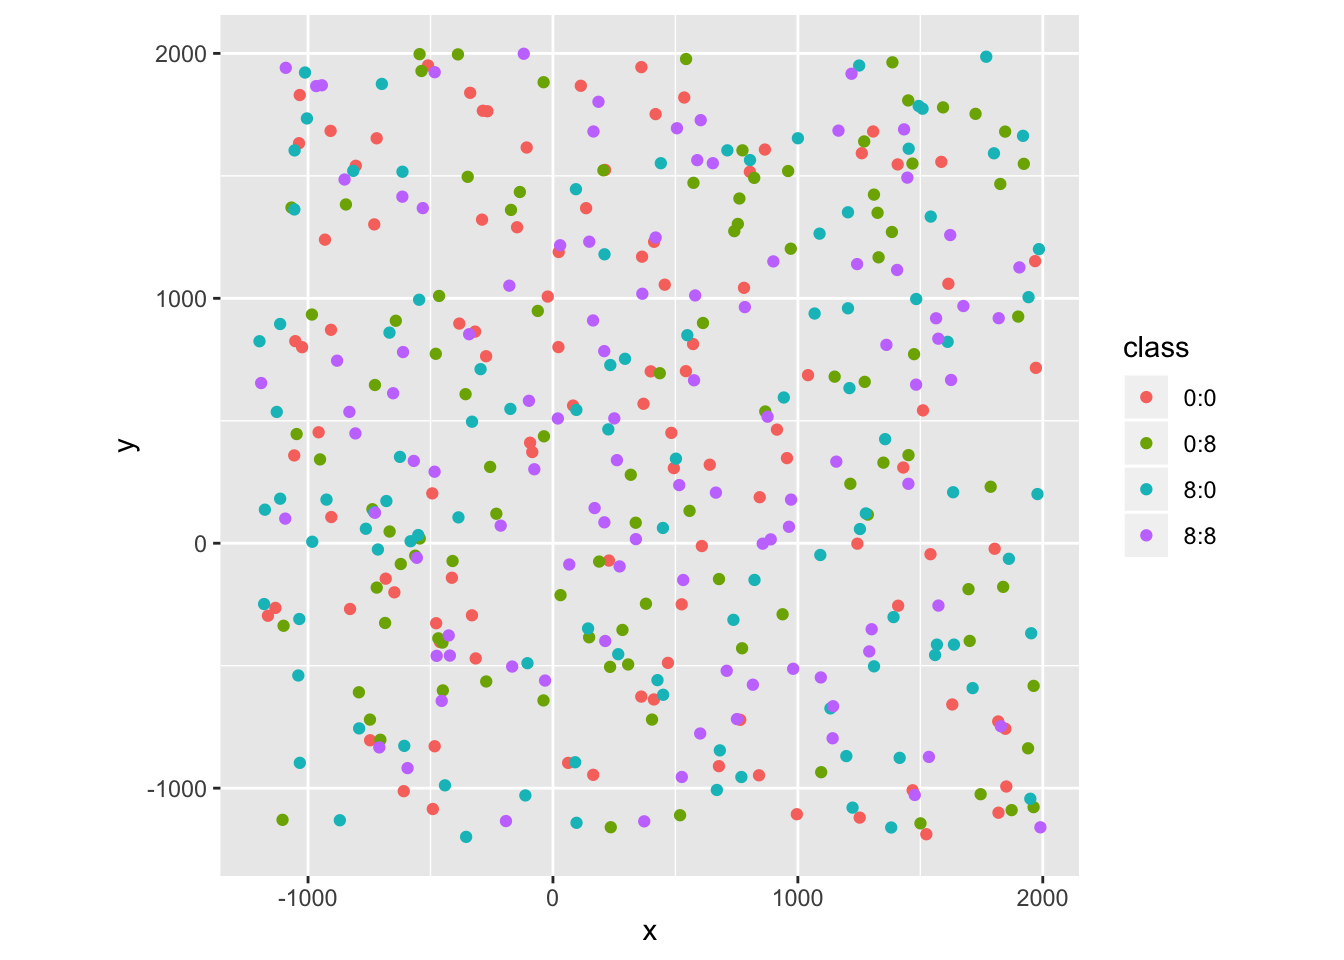
\includegraphics{Chapter4_files/figure-latex/unnamed-chunk-17-1.pdf}

\#\#\#Mixtures greater than two Example: What sort of histogram do we
get when weighing 7,000 canonical nucleotides (A,T,G,C) each type has a
different weight, measured with the same standard deviation sd=3.

\begin{Shaded}
\begin{Highlighting}[]
\NormalTok{masses =}\StringTok{ }\KeywordTok{c}\NormalTok{(}\DataTypeTok{A =}  \DecValTok{331}\NormalTok{, }\DataTypeTok{C =}  \DecValTok{307}\NormalTok{, }\DataTypeTok{G =}  \DecValTok{347}\NormalTok{, }\DataTypeTok{T =}  \DecValTok{322}\NormalTok{)}
\NormalTok{probs  =}\StringTok{ }\KeywordTok{c}\NormalTok{(}\DataTypeTok{A =} \FloatTok{0.12}\NormalTok{, }\DataTypeTok{C =} \FloatTok{0.38}\NormalTok{, }\DataTypeTok{G =} \FloatTok{0.36}\NormalTok{, }\DataTypeTok{T =} \FloatTok{0.14}\NormalTok{)}
\NormalTok{N  =}\StringTok{ }\DecValTok{7000}
\NormalTok{sd =}\StringTok{ }\DecValTok{3}
\NormalTok{nuclt   =}\StringTok{ }\KeywordTok{sample}\NormalTok{(}\KeywordTok{length}\NormalTok{(probs), N, }\DataTypeTok{replace =} \OtherTok{TRUE}\NormalTok{, }\DataTypeTok{prob =}\NormalTok{ probs)}
\NormalTok{quadwts =}\StringTok{ }\KeywordTok{rnorm}\NormalTok{(}\KeywordTok{length}\NormalTok{(nuclt),}
                \DataTypeTok{mean =}\NormalTok{ masses[nuclt],}
                \DataTypeTok{sd   =}\NormalTok{ sd)}
\KeywordTok{ggplot}\NormalTok{(}\KeywordTok{tibble}\NormalTok{(}\DataTypeTok{quadwts =}\NormalTok{ quadwts), }\KeywordTok{aes}\NormalTok{(}\DataTypeTok{x =}\NormalTok{ quadwts)) }\OperatorTok{+}
\StringTok{  }\KeywordTok{geom_histogram}\NormalTok{(}\DataTypeTok{bins =} \DecValTok{100}\NormalTok{, }\DataTypeTok{fill =} \StringTok{"purple"}\NormalTok{)}
\end{Highlighting}
\end{Shaded}

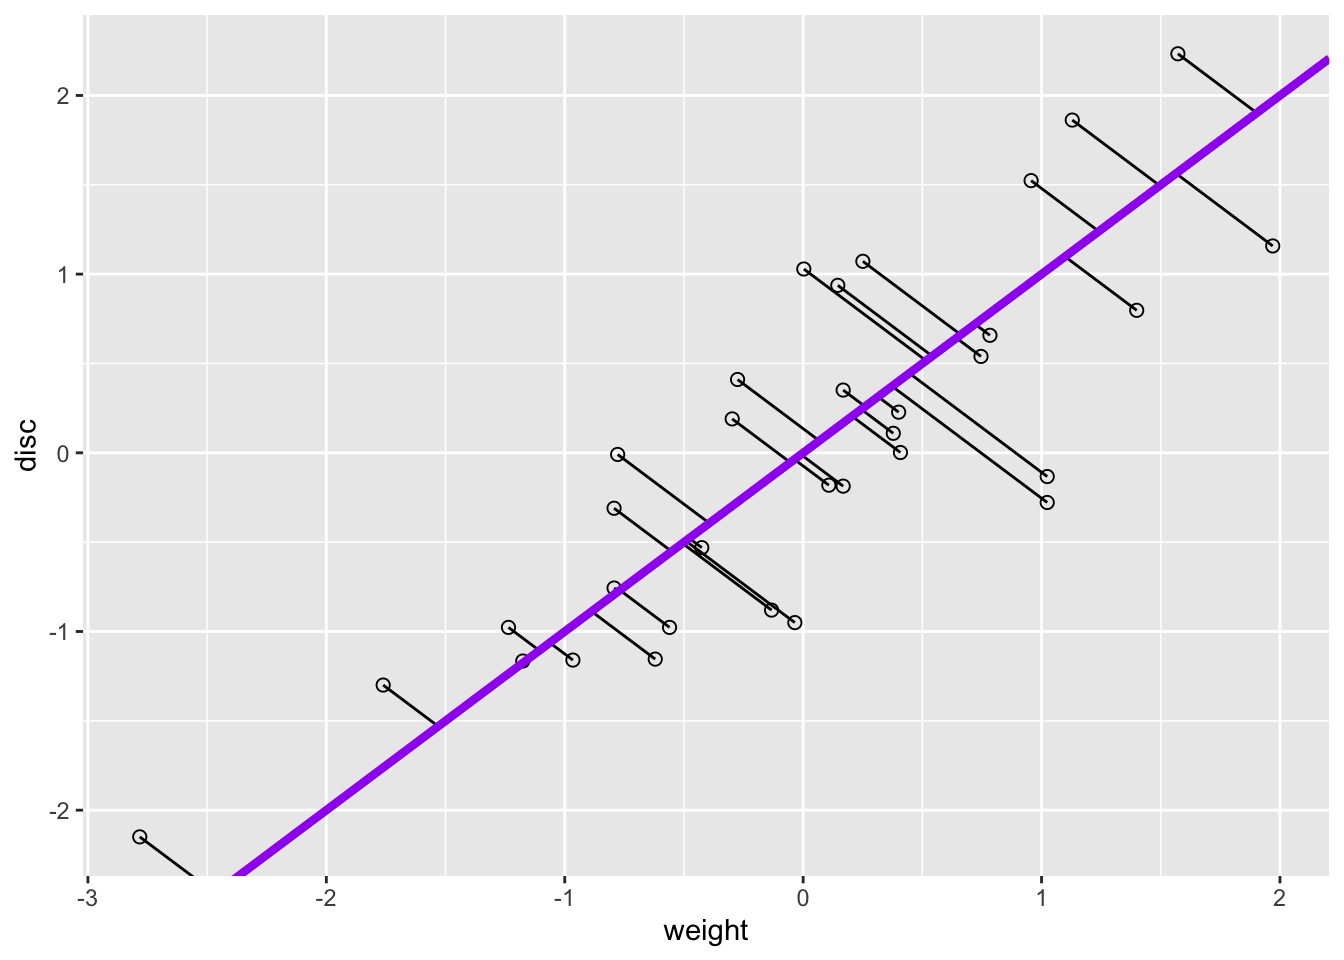
\includegraphics{Chapter4_files/figure-latex/unnamed-chunk-18-1.pdf}

What happens if we repeat this exercise with N=1000 nucleotide
measurements?

\begin{Shaded}
\begin{Highlighting}[]
\NormalTok{N  =}\StringTok{ }\DecValTok{1000}
\NormalTok{sd =}\StringTok{ }\DecValTok{3}
\KeywordTok{set.seed}\NormalTok{(}\DecValTok{1234}\NormalTok{)}
\NormalTok{nuclt   =}\StringTok{ }\KeywordTok{sample}\NormalTok{(}\KeywordTok{length}\NormalTok{(probs), N, }\DataTypeTok{replace =} \OtherTok{TRUE}\NormalTok{, }\DataTypeTok{prob =}\NormalTok{ probs)}
\NormalTok{quadwts =}\StringTok{ }\KeywordTok{rnorm}\NormalTok{(}\KeywordTok{length}\NormalTok{(nuclt),}
                \DataTypeTok{mean =}\NormalTok{ masses[nuclt],}
                \DataTypeTok{sd   =}\NormalTok{ sd)}
\KeywordTok{ggplot}\NormalTok{(}\KeywordTok{tibble}\NormalTok{(}\DataTypeTok{quadwts =}\NormalTok{ quadwts), }\KeywordTok{aes}\NormalTok{(}\DataTypeTok{x =}\NormalTok{ quadwts)) }\OperatorTok{+}
\StringTok{  }\KeywordTok{geom_histogram}\NormalTok{(}\DataTypeTok{bins =} \DecValTok{100}\NormalTok{, }\DataTypeTok{fill =} \StringTok{"purple"}\NormalTok{)}
\end{Highlighting}
\end{Shaded}

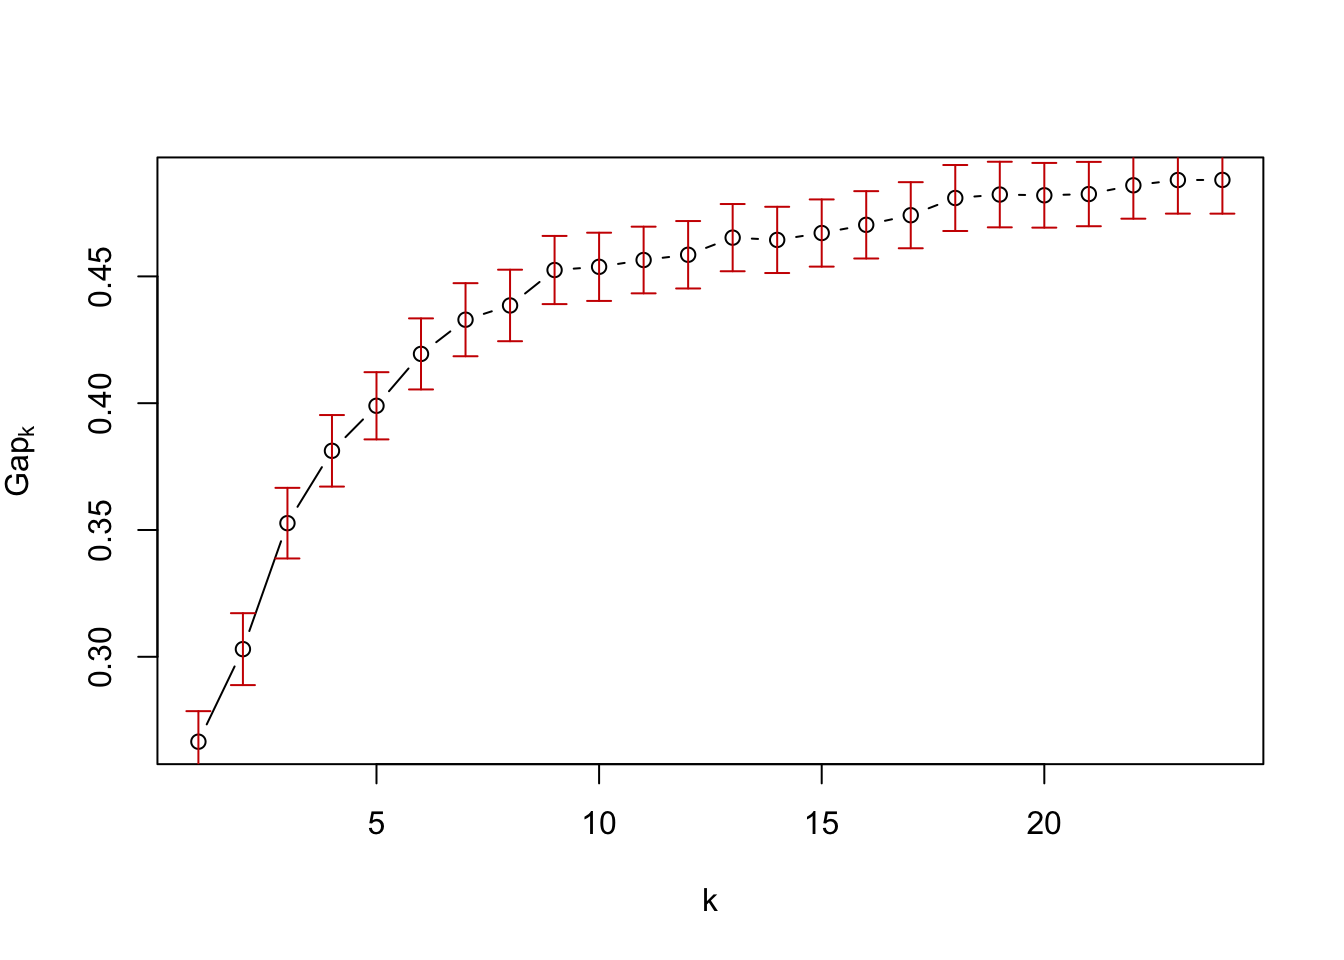
\includegraphics{Chapter4_files/figure-latex/unnamed-chunk-19-1.pdf}

The middle components have become less distinct seeminly indicating just
3 components. this technically an overlap of the mixtures. Lesson:
Increasing the sequence length enhances the dinctinctivness of the
components.

What happens if we keep N=7000 measurements but make the standard
deviation 10?

\begin{Shaded}
\begin{Highlighting}[]
\NormalTok{N  =}\StringTok{ }\DecValTok{7000}
\NormalTok{sd =}\StringTok{ }\DecValTok{10}
\KeywordTok{set.seed}\NormalTok{(}\DecValTok{1234}\NormalTok{)}
\NormalTok{nuclt   =}\StringTok{ }\KeywordTok{sample}\NormalTok{(}\KeywordTok{length}\NormalTok{(probs), N, }\DataTypeTok{replace =} \OtherTok{TRUE}\NormalTok{, }\DataTypeTok{prob =}\NormalTok{ probs)}
\NormalTok{quadwts =}\StringTok{ }\KeywordTok{rnorm}\NormalTok{(}\KeywordTok{length}\NormalTok{(nuclt),}
                \DataTypeTok{mean =}\NormalTok{ masses[nuclt],}
                \DataTypeTok{sd   =}\NormalTok{ sd)}
\KeywordTok{ggplot}\NormalTok{(}\KeywordTok{tibble}\NormalTok{(}\DataTypeTok{quadwts =}\NormalTok{ quadwts), }\KeywordTok{aes}\NormalTok{(}\DataTypeTok{x =}\NormalTok{ quadwts)) }\OperatorTok{+}
\StringTok{  }\KeywordTok{geom_histogram}\NormalTok{(}\DataTypeTok{bins =} \DecValTok{100}\NormalTok{, }\DataTypeTok{fill =} \StringTok{"purple"}\NormalTok{)}
\end{Highlighting}
\end{Shaded}

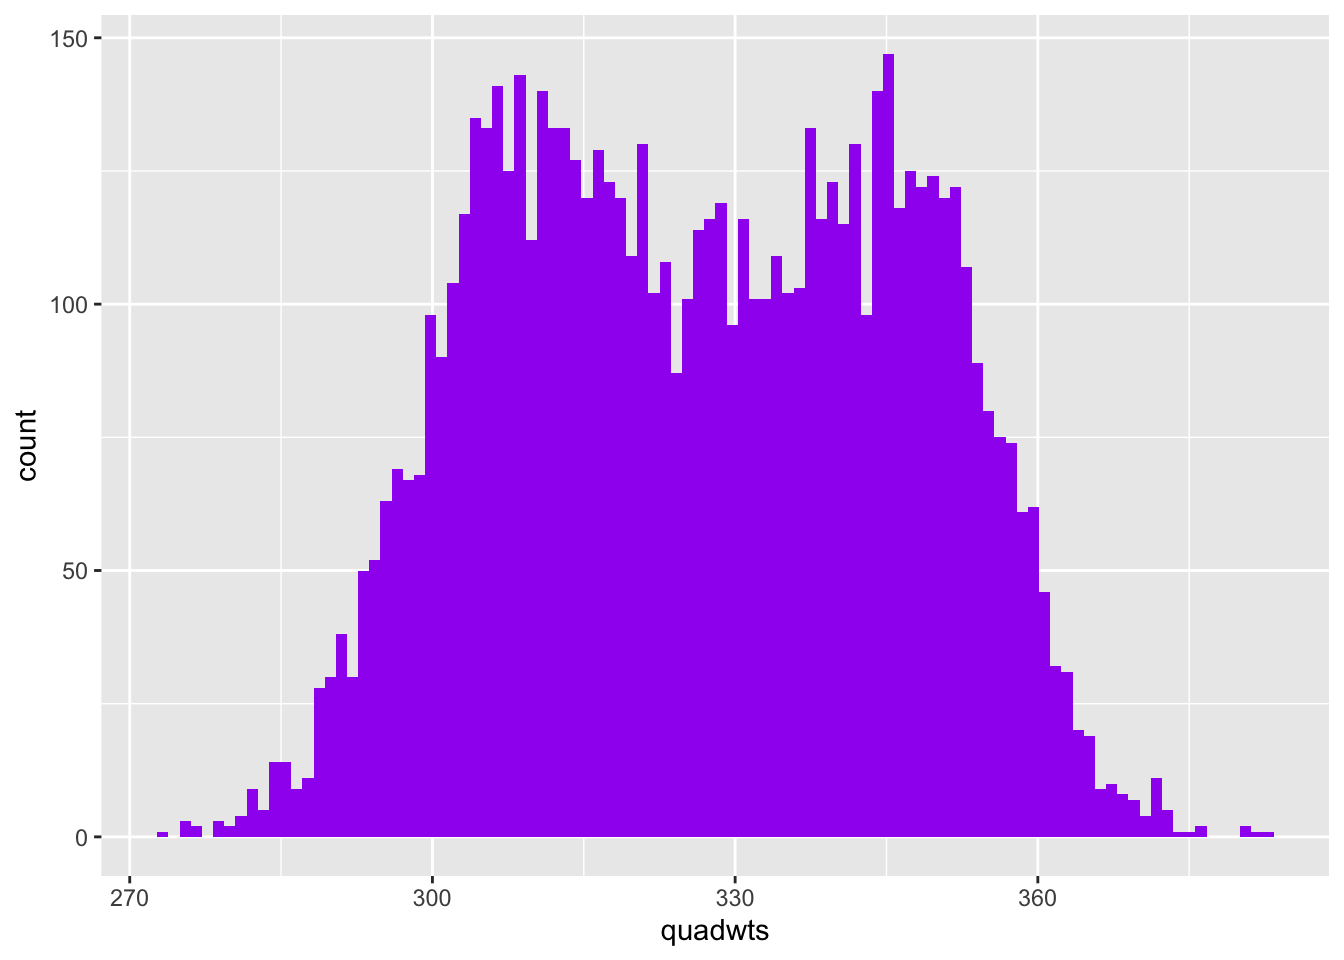
\includegraphics{Chapter4_files/figure-latex/unnamed-chunk-20-1.pdf}

Now the individual components are even less distinct. It looks like
there are only 2 components within our 4 component data. Because
increasing the standard deviation results in mass overlap.

Thus as we have enough measurements with good enough precision, we are
able to distinguish the four nucleotides and decompose the distribution.

\hypertarget{empirical-distributions-and-the-nonparametric-bootstrap}{%
\subsubsection{Empirical distributions and the nonparametric
bootstrap}\label{empirical-distributions-and-the-nonparametric-bootstrap}}

An example is the Darwin's \emph{Zea mays} data where he compared
heights of 15 self-hybridized and 15 self-crossed plants as example.Here
we will consider extreme case of mitxure models, where the number of
observatins is equal to the number of mixture components. An example is
the Darwin's \emph{Zea mays} data where he compared heights of 15
self-hybridized and 15 self-crossed plants as example.

\begin{Shaded}
\begin{Highlighting}[]
\NormalTok{ZeaMays}\OperatorTok{$}\NormalTok{diff}
\end{Highlighting}
\end{Shaded}

\begin{verbatim}
##  [1]  6.125 -8.375  1.000  2.000  0.750  2.875  3.500  5.125  1.750  3.625
## [11]  7.000  3.000  9.375  7.500 -6.000
\end{verbatim}

\begin{Shaded}
\begin{Highlighting}[]
\KeywordTok{ggplot}\NormalTok{(ZeaMays, }\KeywordTok{aes}\NormalTok{(}\DataTypeTok{x =}\NormalTok{ diff, }\DataTypeTok{ymax =} \DecValTok{1}\OperatorTok{/}\DecValTok{15}\NormalTok{, }\DataTypeTok{ymin =} \DecValTok{0}\NormalTok{)) }\OperatorTok{+}
\StringTok{  }\KeywordTok{geom_linerange}\NormalTok{(}\DataTypeTok{size =} \DecValTok{1}\NormalTok{, }\DataTypeTok{col =} \StringTok{"forestgreen"}\NormalTok{) }\OperatorTok{+}\StringTok{ }\KeywordTok{ylim}\NormalTok{(}\DecValTok{0}\NormalTok{, }\FloatTok{0.1}\NormalTok{)}
\end{Highlighting}
\end{Shaded}

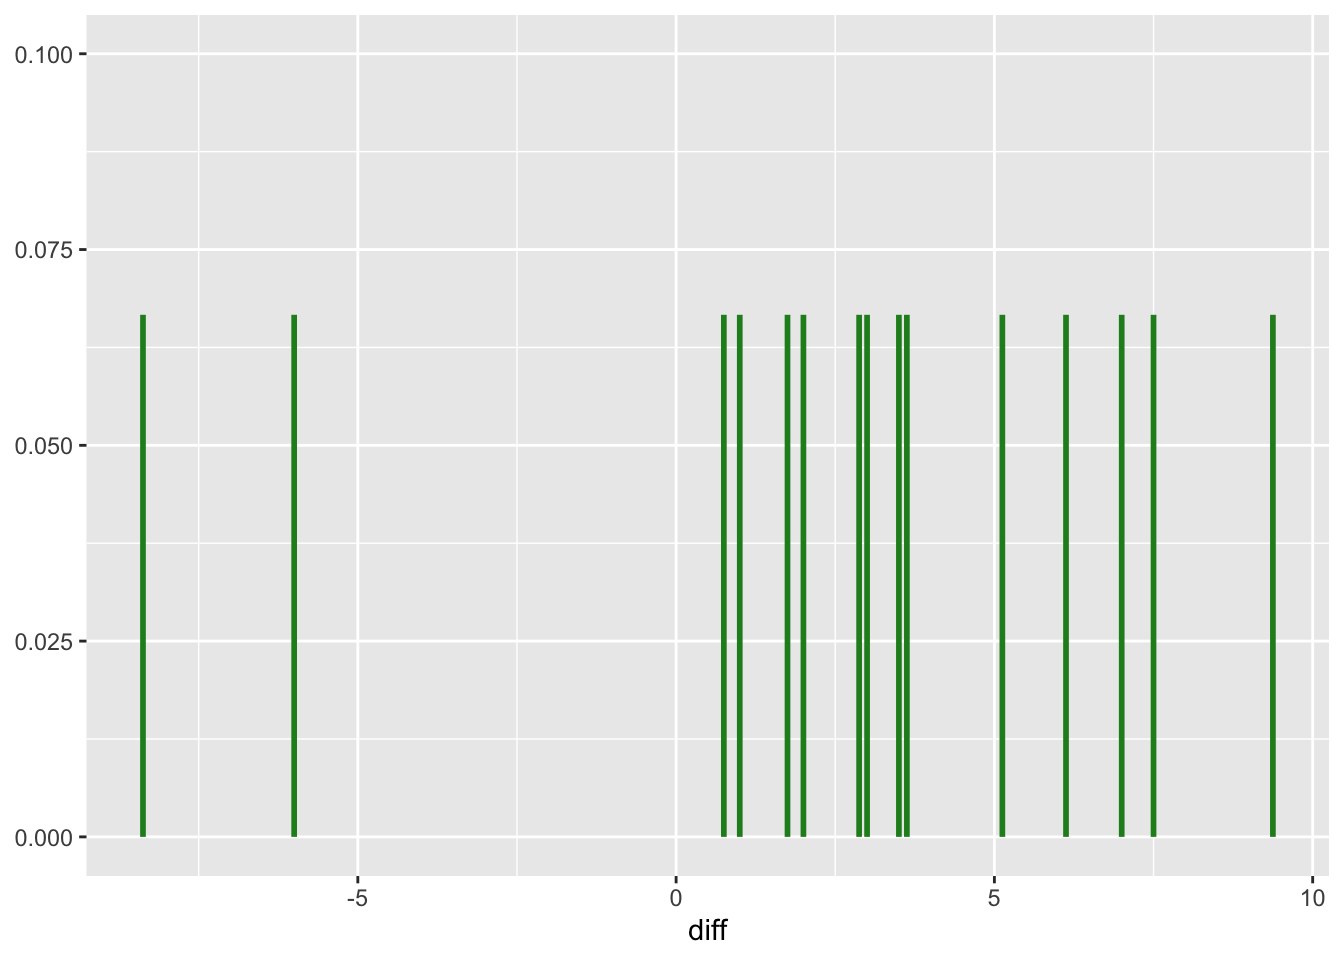
\includegraphics{Chapter4_files/figure-latex/unnamed-chunk-21-1.pdf}

We can bootstrap to estimate the sampling distribution of the median of
the Zea Mays differences.

\begin{Shaded}
\begin{Highlighting}[]
\KeywordTok{set.seed}\NormalTok{(}\DecValTok{1234}\NormalTok{)}
\NormalTok{B =}\StringTok{ }\DecValTok{1000}
\NormalTok{meds =}\StringTok{ }\KeywordTok{replicate}\NormalTok{(B, \{}
\NormalTok{  i =}\StringTok{ }\KeywordTok{sample}\NormalTok{(}\DecValTok{15}\NormalTok{, }\DecValTok{15}\NormalTok{, }\DataTypeTok{replace =} \OtherTok{TRUE}\NormalTok{)}
  \KeywordTok{median}\NormalTok{(ZeaMays}\OperatorTok{$}\NormalTok{diff[i])}
\NormalTok{\})}
\KeywordTok{ggplot}\NormalTok{(}\KeywordTok{tibble}\NormalTok{(}\DataTypeTok{medians =}\NormalTok{ meds), }\KeywordTok{aes}\NormalTok{(}\DataTypeTok{x =}\NormalTok{ medians)) }\OperatorTok{+}
\StringTok{  }\KeywordTok{geom_histogram}\NormalTok{(}\DataTypeTok{bins =} \DecValTok{30}\NormalTok{, }\DataTypeTok{fill =} \StringTok{"purple"}\NormalTok{)}
\end{Highlighting}
\end{Shaded}

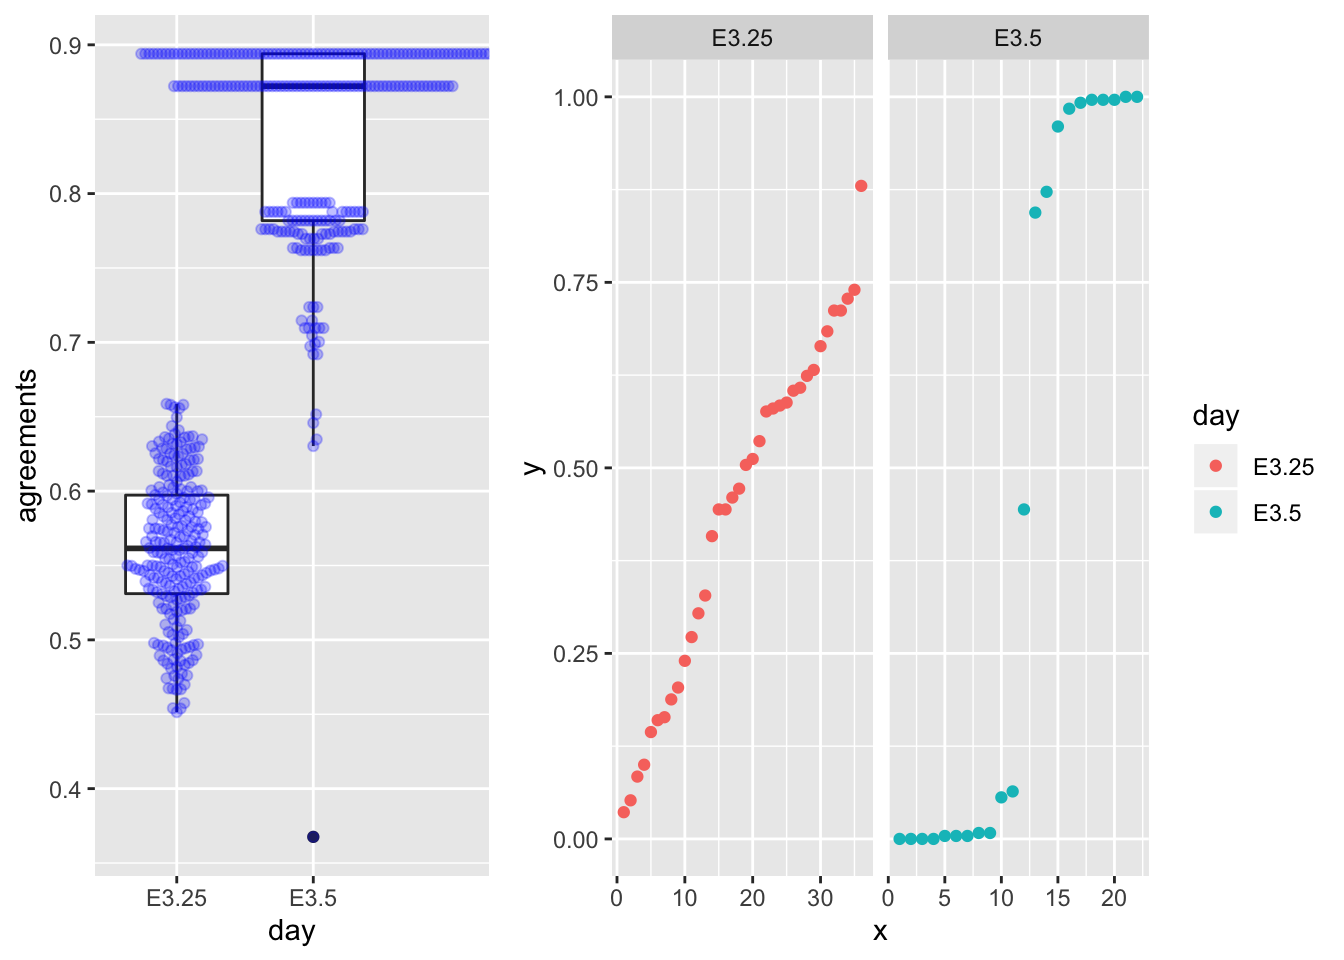
\includegraphics{Chapter4_files/figure-latex/unnamed-chunk-22-1.pdf}

We can also estimate a 99\% confidence interval for the median based on
these simulations. The quantile function can be used for this.

\begin{Shaded}
\begin{Highlighting}[]
\KeywordTok{quantile}\NormalTok{(meds,}\KeywordTok{c}\NormalTok{(}\FloatTok{0.005}\NormalTok{,}\FloatTok{0.995}\NormalTok{))}
\end{Highlighting}
\end{Shaded}

\begin{verbatim}
##    0.5%   99.5% 
## 0.99875 6.12500
\end{verbatim}

Use the bootstrap package to redo the same analysis using the function
bootstrap for both median and mean. What differences do you notice
between the sampling distribution of the mean and the median?

\begin{Shaded}
\begin{Highlighting}[]
\NormalTok{boot_means=}\KeywordTok{bootstrap}\NormalTok{(ZeaMays}\OperatorTok{$}\NormalTok{diff, B, mean)}
\NormalTok{boot_medians=}\KeywordTok{bootstrap}\NormalTok{(ZeaMays}\OperatorTok{$}\NormalTok{diff, B, median)}
\end{Highlighting}
\end{Shaded}

\begin{Shaded}
\begin{Highlighting}[]
\KeywordTok{ggplot}\NormalTok{(}\KeywordTok{tibble}\NormalTok{(boot_means}\OperatorTok{$}\NormalTok{thetastar),}\KeywordTok{aes}\NormalTok{(}\DataTypeTok{x =}\NormalTok{ boot_means}\OperatorTok{$}\NormalTok{thetastar))}\OperatorTok{+}
\StringTok{  }\KeywordTok{geom_histogram}\NormalTok{(}\DataTypeTok{bins =} \DecValTok{30}\NormalTok{, }\DataTypeTok{fill =} \StringTok{"purple"}\NormalTok{)}
\end{Highlighting}
\end{Shaded}

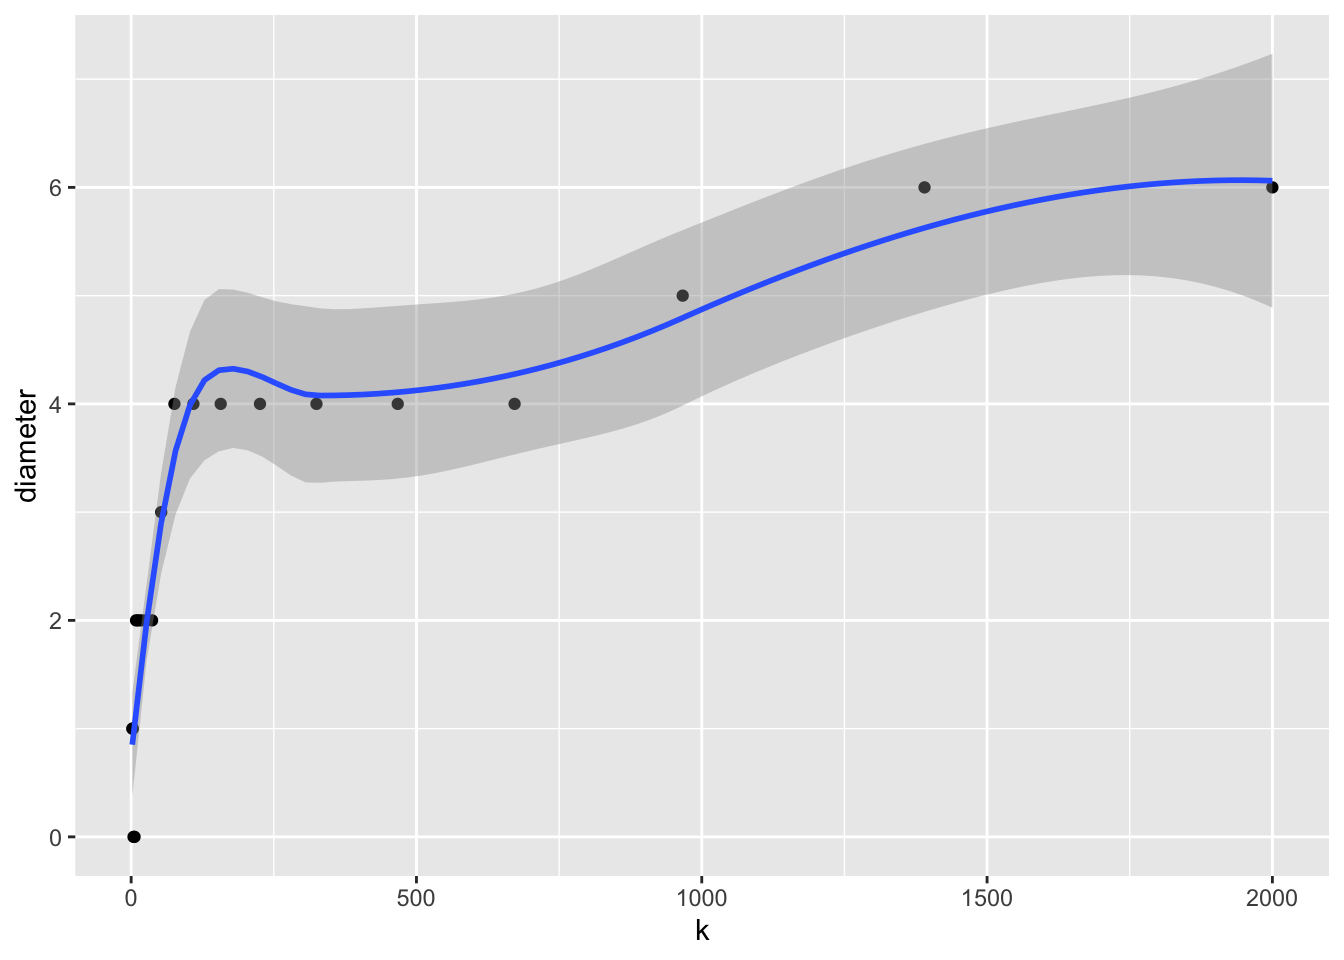
\includegraphics{Chapter4_files/figure-latex/unnamed-chunk-25-1.pdf}

\begin{Shaded}
\begin{Highlighting}[]
\KeywordTok{ggplot}\NormalTok{(}\KeywordTok{tibble}\NormalTok{(boot_medians}\OperatorTok{$}\NormalTok{thetastar),}\KeywordTok{aes}\NormalTok{(}\DataTypeTok{x =}\NormalTok{ boot_medians}\OperatorTok{$}\NormalTok{thetastar))}\OperatorTok{+}
\StringTok{  }\KeywordTok{geom_histogram}\NormalTok{(}\DataTypeTok{bins =} \DecValTok{30}\NormalTok{, }\DataTypeTok{fill =} \StringTok{"purple"}\NormalTok{)}
\end{Highlighting}
\end{Shaded}

\includegraphics{Chapter4_files/figure-latex/unnamed-chunk-25-2.pdf}

The bootstrap uses a mixture with n components, so with a sample of size
n, it qualifies as a nonparametric method. If the sample is composed of
n=3 different values, how many different bootstrap resamples are
possible? Answer the same question with n = 15.

\begin{Shaded}
\begin{Highlighting}[]
\KeywordTok{c}\NormalTok{(}\DataTypeTok{N3 =} \KeywordTok{choose}\NormalTok{(}\DecValTok{5}\NormalTok{, }\DecValTok{3}\NormalTok{), }\DataTypeTok{N15 =} \KeywordTok{choose}\NormalTok{(}\DecValTok{29}\NormalTok{, }\DecValTok{15}\NormalTok{))}
\end{Highlighting}
\end{Shaded}

\begin{verbatim}
##       N3      N15 
##       10 77558760
\end{verbatim}

\#\#\#Infinite Mixtures

\#\#Infinite mixture of normals

This is when the number of mixture components is greater than or equal
to the number of observations.

Let's simulate an infinite mixture using a 2 level of data generation
technique. In level 1, we generate 10000 random deviates (w) from the
exponential distribution with rate (ie. mean) equal to 1. In level 2,
the deviates (w) serve as the variances of normal variables with mean μ
generated using rnorm. We finally visualize the data.

\begin{Shaded}
\begin{Highlighting}[]
\NormalTok{w =}\StringTok{ }\KeywordTok{rexp}\NormalTok{(}\DecValTok{10000}\NormalTok{, }\DataTypeTok{rate =} \DecValTok{1}\NormalTok{)}
\NormalTok{mu  =}\StringTok{ }\FloatTok{0.3}
\NormalTok{lps =}\StringTok{ }\KeywordTok{rnorm}\NormalTok{(}\KeywordTok{length}\NormalTok{(w), }\DataTypeTok{mean =}\NormalTok{ mu, }\DataTypeTok{sd =} \KeywordTok{sqrt}\NormalTok{(w))}
\KeywordTok{ggplot}\NormalTok{(}\KeywordTok{data.frame}\NormalTok{(lps), }\KeywordTok{aes}\NormalTok{(}\DataTypeTok{x =}\NormalTok{ lps)) }\OperatorTok{+}
\StringTok{  }\KeywordTok{geom_histogram}\NormalTok{(}\DataTypeTok{fill =} \StringTok{"purple"}\NormalTok{, }\DataTypeTok{binwidth =} \FloatTok{0.1}\NormalTok{)}
\end{Highlighting}
\end{Shaded}

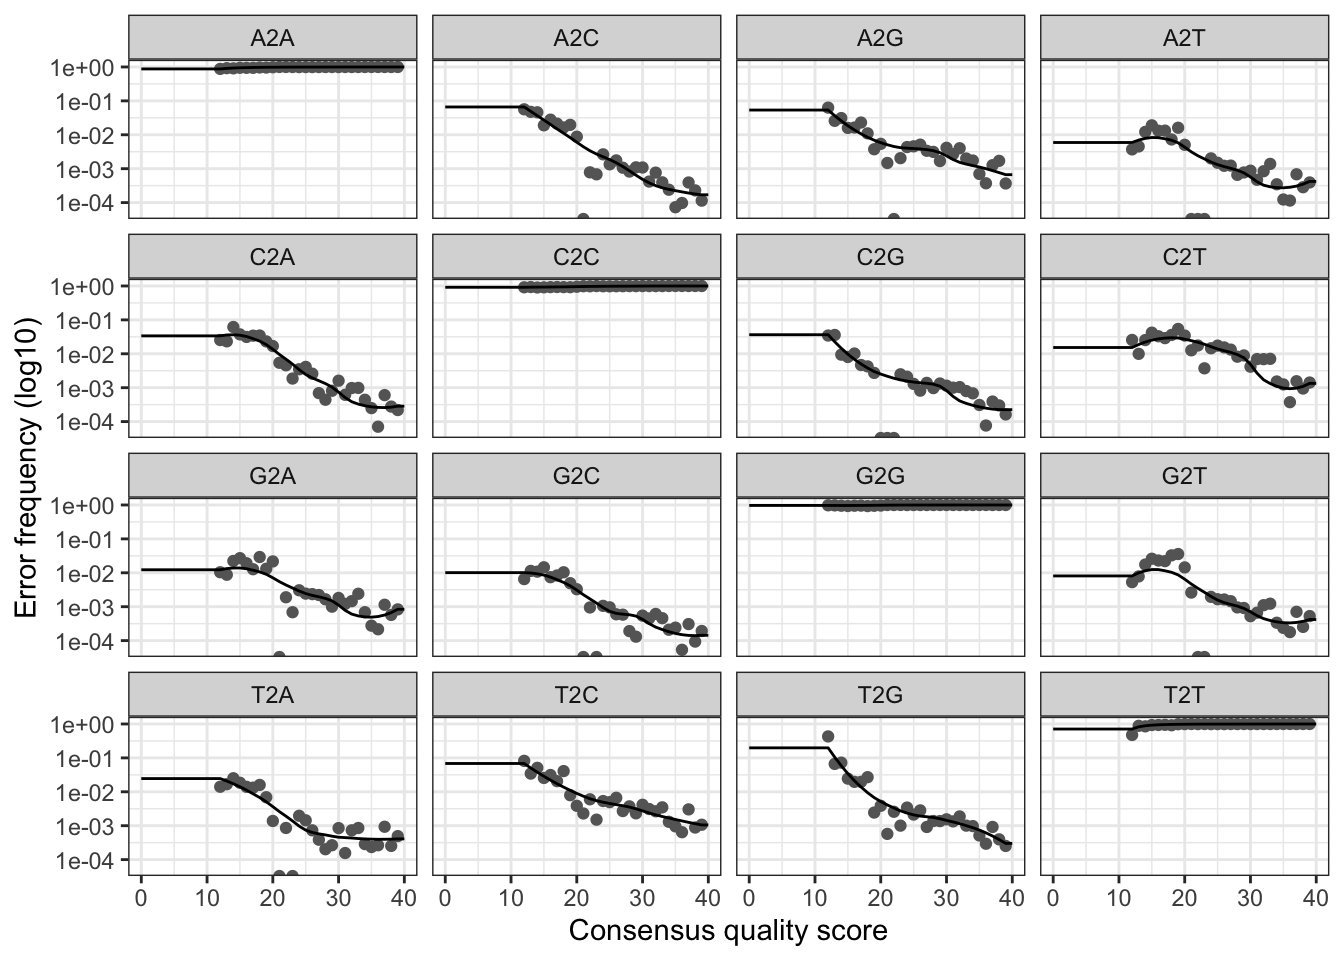
\includegraphics{Chapter4_files/figure-latex/unnamed-chunk-27-1.pdf}

This is called a \emph{Laplace distribution}. It is useful because
\emph{the median is a good estimator of its location parameter θ}. and
that the \emph{its scale parameter ϕ can be estimated from the median
absolute deviation}.

\#\#\#Asymmetric Laplace In the Laplace distribution, the variances of
the normal components depend on W, while the means are unaffected. Lets
generate and visualize data from an asymmetric Laplace distribution.

\begin{Shaded}
\begin{Highlighting}[]
\NormalTok{mu =}\StringTok{ }\FloatTok{0.3}\NormalTok{; sigma =}\StringTok{ }\FloatTok{0.4}\NormalTok{; theta =}\StringTok{ }\DecValTok{-1}
\NormalTok{w  =}\StringTok{ }\KeywordTok{rexp}\NormalTok{(}\DecValTok{10000}\NormalTok{, }\DecValTok{1}\NormalTok{)}
\NormalTok{alps =}\StringTok{ }\KeywordTok{rnorm}\NormalTok{(}\KeywordTok{length}\NormalTok{(w), theta }\OperatorTok{+}\StringTok{ }\NormalTok{mu }\OperatorTok{*}\StringTok{ }\NormalTok{w, sigma }\OperatorTok{*}\StringTok{ }\KeywordTok{sqrt}\NormalTok{(w))}
\KeywordTok{ggplot}\NormalTok{(}\KeywordTok{tibble}\NormalTok{(alps), }\KeywordTok{aes}\NormalTok{(}\DataTypeTok{x =}\NormalTok{ alps)) }\OperatorTok{+}
\StringTok{  }\KeywordTok{geom_histogram}\NormalTok{(}\DataTypeTok{fill =} \StringTok{"purple"}\NormalTok{, }\DataTypeTok{binwidth =} \FloatTok{0.1}\NormalTok{)}
\end{Highlighting}
\end{Shaded}

\includegraphics{Chapter4_files/figure-latex/unnamed-chunk-28-1.pdf}

\begin{Shaded}
\begin{Highlighting}[]
\NormalTok{knitr}\OperatorTok{::}\KeywordTok{include_graphics}\NormalTok{(}\KeywordTok{c}\NormalTok{(}\StringTok{'images/LaplaceMixturePromoterLengths.png'}\NormalTok{,}\StringTok{'images/tcellhist.png'}\NormalTok{))}
\end{Highlighting}
\end{Shaded}

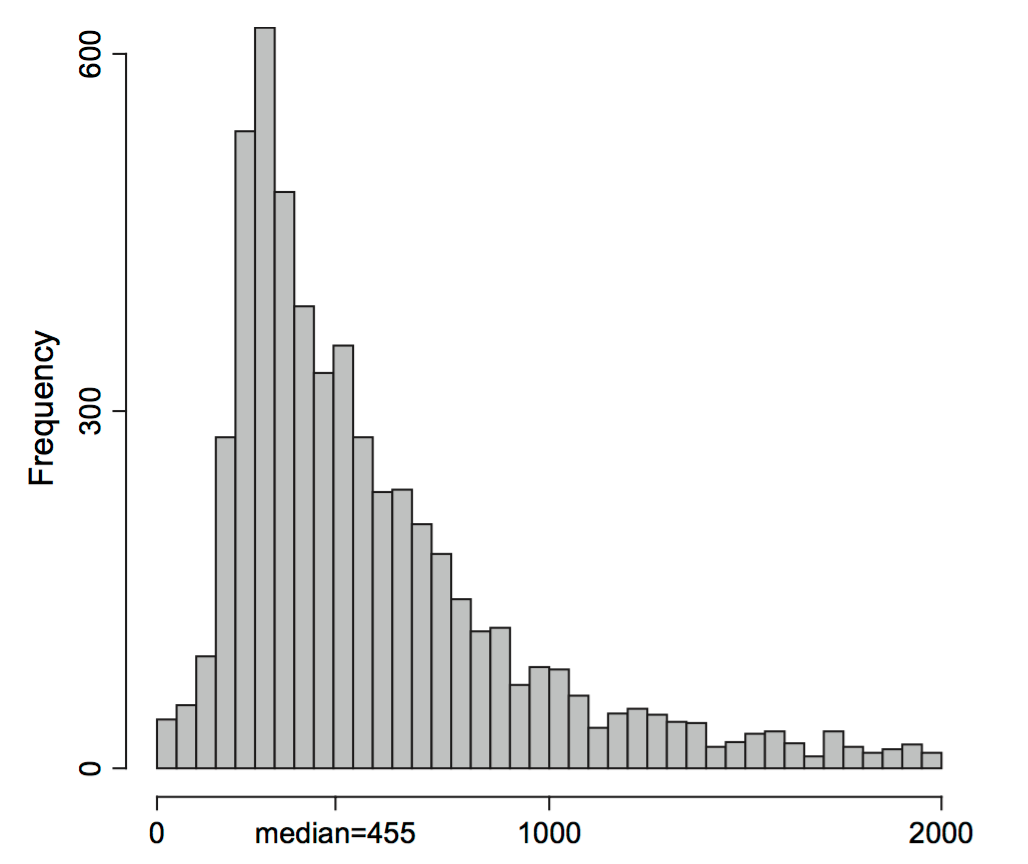
\includegraphics{images/LaplaceMixturePromoterLengths.png}
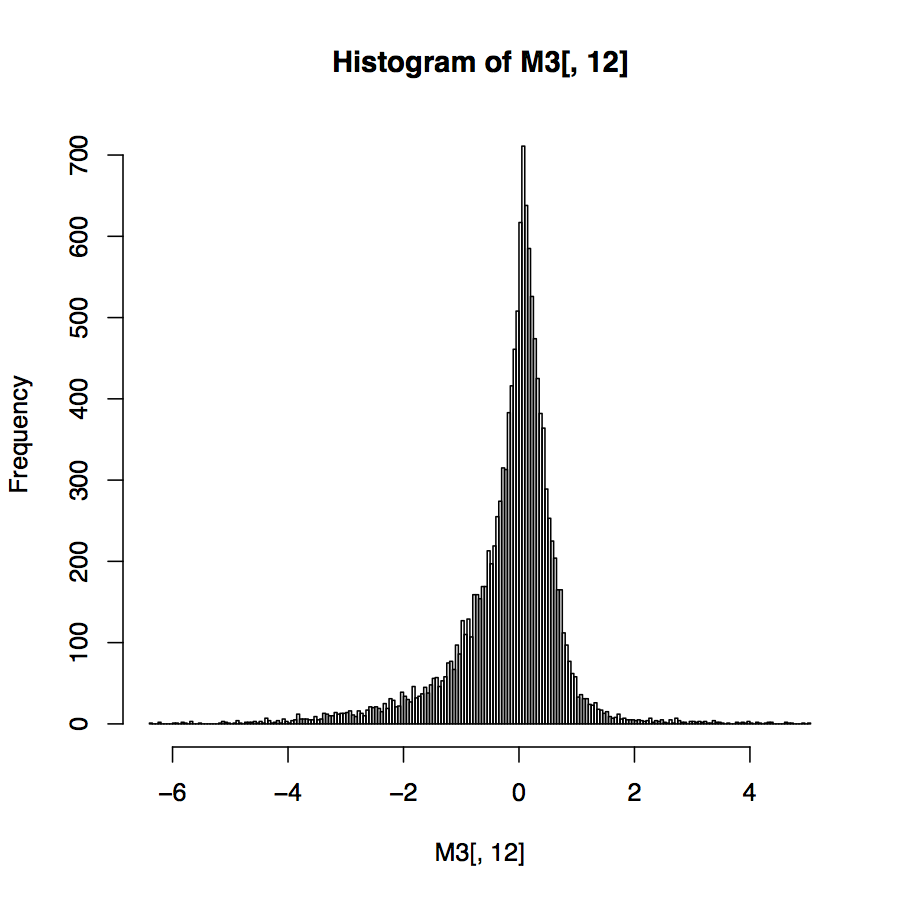
\includegraphics{images/tcellhist.png}

\hypertarget{infinite-mixtures-of-poisson-variables-the-case-of-gamma-poisson-distribution}{%
\subsection{Infinite mixtures of poisson variables: the case of
gamma-poisson
distribution}\label{infinite-mixtures-of-poisson-variables-the-case-of-gamma-poisson-distribution}}

modelling a real-world count data requires a two-level hierarchical
model where simple Poisson and binomial distributions serve as the
building blocks at the lower level. Examples of sampling schemes that
are well modeled by mixtures of Poisson variables include RNA-Seq, and
16S rRNA-Seq data used in microbial ecology.

\#\#\#Gamma distribution: two parameters (shape and scale) The gamma
distribution is an extension of the (one-parameter) exponential
distribution, but it has two parameters, which makes it more flexible.
It is often useful as a building block for the upper level of a
hierarchical model.

Example gamma distributions

\begin{Shaded}
\begin{Highlighting}[]
\KeywordTok{set.seed}\NormalTok{(}\DecValTok{1234}\NormalTok{)}
\KeywordTok{ggplot}\NormalTok{(}\KeywordTok{tibble}\NormalTok{(}\DataTypeTok{x =} \KeywordTok{rgamma}\NormalTok{(}\DecValTok{10000}\NormalTok{, }\DataTypeTok{shape =} \DecValTok{2}\NormalTok{, }\DataTypeTok{rate =} \DecValTok{1}\OperatorTok{/}\DecValTok{3}\NormalTok{)),}
   \KeywordTok{aes}\NormalTok{(}\DataTypeTok{x =}\NormalTok{ x)) }\OperatorTok{+}\StringTok{ }\KeywordTok{geom_histogram}\NormalTok{(}\DataTypeTok{bins =} \DecValTok{100}\NormalTok{, }\DataTypeTok{fill=} \StringTok{"purple"}\NormalTok{)}
\end{Highlighting}
\end{Shaded}

\includegraphics{Chapter4_files/figure-latex/unnamed-chunk-30-1.pdf}

\begin{Shaded}
\begin{Highlighting}[]
\KeywordTok{ggplot}\NormalTok{(}\KeywordTok{tibble}\NormalTok{(}\DataTypeTok{x =} \KeywordTok{rgamma}\NormalTok{(}\DecValTok{10000}\NormalTok{, }\DataTypeTok{shape =} \DecValTok{10}\NormalTok{, }\DataTypeTok{rate =} \DecValTok{3}\OperatorTok{/}\DecValTok{2}\NormalTok{)),}
   \KeywordTok{aes}\NormalTok{(}\DataTypeTok{x =}\NormalTok{ x)) }\OperatorTok{+}\StringTok{ }\KeywordTok{geom_histogram}\NormalTok{(}\DataTypeTok{bins =} \DecValTok{100}\NormalTok{, }\DataTypeTok{fill=} \StringTok{"purple"}\NormalTok{)}
\end{Highlighting}
\end{Shaded}

\includegraphics{Chapter4_files/figure-latex/unnamed-chunk-30-2.pdf}

Example gamma-Poisson hierachical model

\begin{Shaded}
\begin{Highlighting}[]
\NormalTok{lambda =}\StringTok{ }\KeywordTok{rgamma}\NormalTok{(}\DecValTok{10000}\NormalTok{, }\DataTypeTok{shape =} \DecValTok{10}\NormalTok{, }\DataTypeTok{rate =} \DecValTok{3}\OperatorTok{/}\DecValTok{2}\NormalTok{)}
\NormalTok{gp =}\StringTok{ }\KeywordTok{rpois}\NormalTok{(}\KeywordTok{length}\NormalTok{(lambda), }\DataTypeTok{lambda =}\NormalTok{ lambda)}
\KeywordTok{ggplot}\NormalTok{(}\KeywordTok{tibble}\NormalTok{(}\DataTypeTok{x =}\NormalTok{ gp), }\KeywordTok{aes}\NormalTok{(}\DataTypeTok{x =}\NormalTok{ x)) }\OperatorTok{+}
\StringTok{  }\KeywordTok{geom_histogram}\NormalTok{(}\DataTypeTok{bins =} \DecValTok{100}\NormalTok{, }\DataTypeTok{fill=} \StringTok{"purple"}\NormalTok{)}
\end{Highlighting}
\end{Shaded}

\includegraphics{Chapter4_files/figure-latex/unnamed-chunk-31-1.pdf} The
Gamma-Poisson distribution is a discrete distribution. Gamma-Poisson
distribution is also called \emph{negative binomial distribution}.
Formula for equation is similar to binomial distribution Gamma-Poisson
is more defining of the underlying principles

\begin{Shaded}
\begin{Highlighting}[]
\NormalTok{ofit =}\StringTok{ }\KeywordTok{goodfit}\NormalTok{(gp, }\StringTok{"nbinomial"}\NormalTok{)}
\KeywordTok{plot}\NormalTok{(ofit, }\DataTypeTok{xlab =} \StringTok{""}\NormalTok{)}
\end{Highlighting}
\end{Shaded}

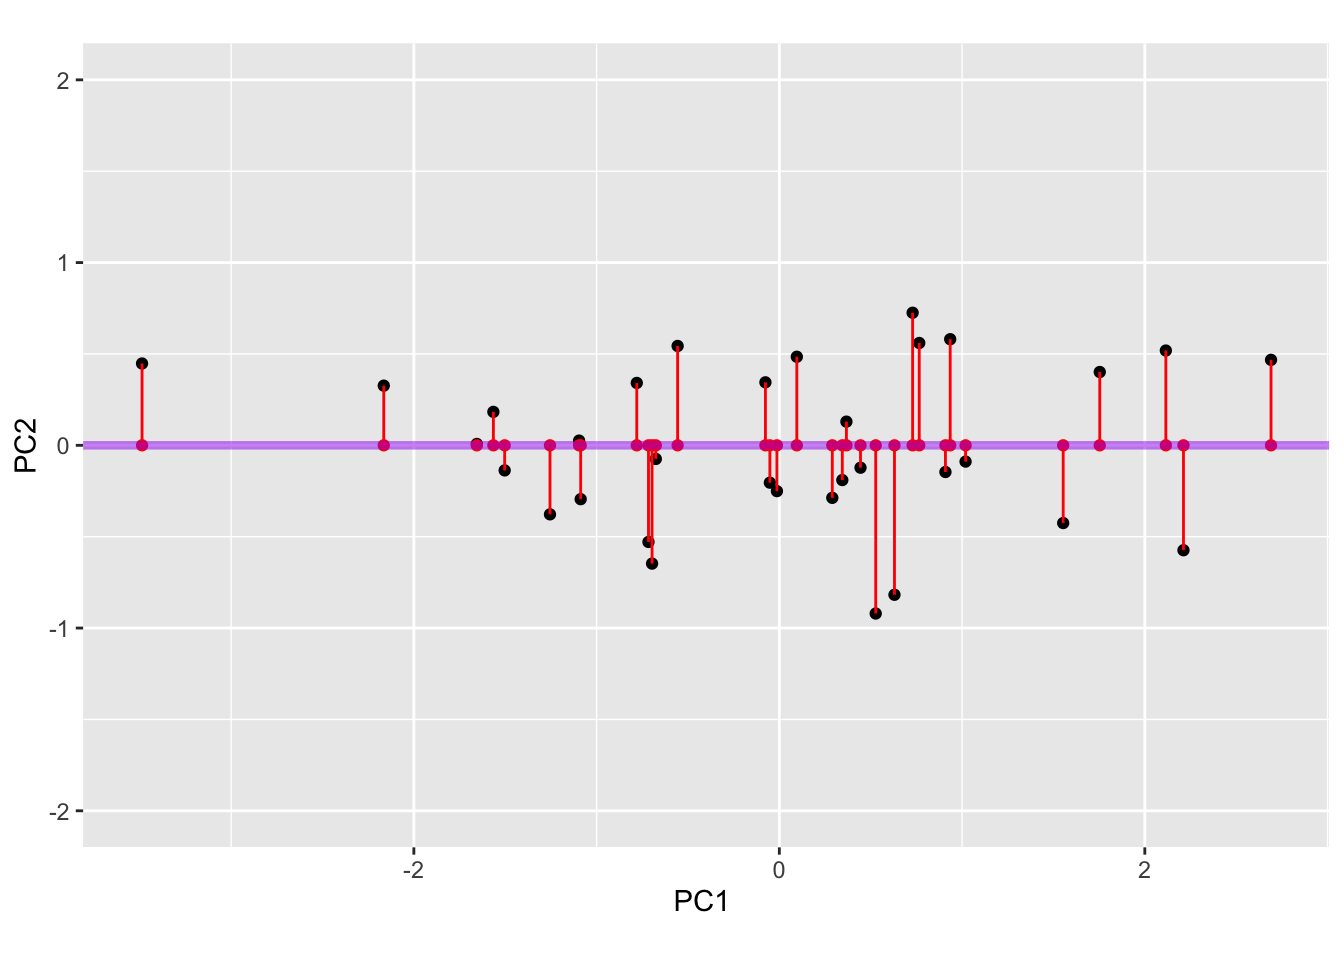
\includegraphics{Chapter4_files/figure-latex/unnamed-chunk-32-1.pdf}

\begin{Shaded}
\begin{Highlighting}[]
\NormalTok{ofit}\OperatorTok{$}\NormalTok{par}
\end{Highlighting}
\end{Shaded}

\begin{verbatim}
## $size
## [1] 9.970598
## 
## $prob
## [1] 0.5998435
\end{verbatim}

\#\#\#Variance stabilizing transformations Transformations are important
in reducing the heterogeneity and heteroscedasticity of the data. The
goal is to stabilze the variance. Instability in the variance is a
source of noise. Example of simulated data before and after
transformation

\begin{Shaded}
\begin{Highlighting}[]
\KeywordTok{set.seed}\NormalTok{(}\DecValTok{1234}\NormalTok{)}
\NormalTok{lambdas =}\StringTok{ }\KeywordTok{seq}\NormalTok{(}\DecValTok{100}\NormalTok{, }\DecValTok{900}\NormalTok{, }\DataTypeTok{by =} \DecValTok{100}\NormalTok{)}
\NormalTok{simdat =}\StringTok{ }\KeywordTok{lapply}\NormalTok{(lambdas, }\ControlFlowTok{function}\NormalTok{(l)}
    \KeywordTok{tibble}\NormalTok{(}\DataTypeTok{y =} \KeywordTok{rpois}\NormalTok{(}\DataTypeTok{n =} \DecValTok{40}\NormalTok{, }\DataTypeTok{lambda=}\NormalTok{l), }\DataTypeTok{lambda =}\NormalTok{ l)}
\NormalTok{  ) }\OperatorTok\StringTok{ }\NormalTok{bind_rows}
\CommentTok{#data before transformation}
\KeywordTok{ggplot}\NormalTok{(simdat, }\KeywordTok{aes}\NormalTok{(}\DataTypeTok{x =}\NormalTok{ lambda, }\DataTypeTok{y =}\NormalTok{ y)) }\OperatorTok{+}
\StringTok{  }\KeywordTok{geom_beeswarm}\NormalTok{(}\DataTypeTok{alpha =} \FloatTok{0.6}\NormalTok{, }\DataTypeTok{color =} \StringTok{"purple"}\NormalTok{)}
\end{Highlighting}
\end{Shaded}

\includegraphics{Chapter4_files/figure-latex/unnamed-chunk-33-1.pdf}

\begin{Shaded}
\begin{Highlighting}[]
\CommentTok{#data after square root transformation}
\KeywordTok{ggplot}\NormalTok{(simdat, }\KeywordTok{aes}\NormalTok{(}\DataTypeTok{x =}\NormalTok{ lambda, }\DataTypeTok{y =} \KeywordTok{sqrt}\NormalTok{(y))) }\OperatorTok{+}
\StringTok{  }\KeywordTok{geom_beeswarm}\NormalTok{(}\DataTypeTok{alpha =} \FloatTok{0.6}\NormalTok{, }\DataTypeTok{color =} \StringTok{"purple"}\NormalTok{)}
\end{Highlighting}
\end{Shaded}

\includegraphics{Chapter4_files/figure-latex/unnamed-chunk-33-2.pdf}

\begin{Shaded}
\begin{Highlighting}[]
\NormalTok{.o =}\StringTok{ }\KeywordTok{options}\NormalTok{(}\DataTypeTok{digits =} \DecValTok{3}\NormalTok{)}
\KeywordTok{summarise}\NormalTok{(}\KeywordTok{group_by}\NormalTok{(simdat, lambda), }\KeywordTok{sd}\NormalTok{(y), }\KeywordTok{sd}\NormalTok{(}\DecValTok{2}\OperatorTok{*}\KeywordTok{sqrt}\NormalTok{(y)))}
\end{Highlighting}
\end{Shaded}

\begin{verbatim}
## # A tibble: 9 x 3
##   lambda `sd(y)` `sd(2 * sqrt(y))`
##    <dbl>   <dbl>             <dbl>
## 1    100    10.1             0.996
## 2    200    15.4             1.06 
## 3    300    15.5             0.903
## 4    400    18.3             0.913
## 5    500    23.6             1.05 
## 6    600    23.6             0.959
## 7    700    25.6             0.965
## 8    800    31.2             1.10 
## 9    900    32.9             1.10
\end{verbatim}

\begin{Shaded}
\begin{Highlighting}[]
\KeywordTok{options}\NormalTok{(.o)}
\end{Highlighting}
\end{Shaded}

Repeat the computation in the above code chunk for a version of simdat
with a larger number of replicates than 40.

\begin{Shaded}
\begin{Highlighting}[]
\KeywordTok{set.seed}\NormalTok{(}\DecValTok{1234}\NormalTok{)}
\NormalTok{lambdas =}\StringTok{ }\KeywordTok{seq}\NormalTok{(}\DecValTok{100}\NormalTok{, }\DecValTok{900}\NormalTok{, }\DataTypeTok{by =} \DecValTok{100}\NormalTok{)}
\NormalTok{simdat2 =}\StringTok{ }\KeywordTok{lapply}\NormalTok{(lambdas, }\ControlFlowTok{function}\NormalTok{(l)}
    \KeywordTok{tibble}\NormalTok{(}\DataTypeTok{y =} \KeywordTok{rpois}\NormalTok{(}\DataTypeTok{n =} \DecValTok{1000}\NormalTok{, }\DataTypeTok{lambda=}\NormalTok{l), }\DataTypeTok{lambda =}\NormalTok{ l)}
\NormalTok{  ) }\OperatorTok\StringTok{ }\NormalTok{bind_rows}
\CommentTok{#data before transformation}
\KeywordTok{ggplot}\NormalTok{(simdat2, }\KeywordTok{aes}\NormalTok{(}\DataTypeTok{x =}\NormalTok{ lambda, }\DataTypeTok{y =}\NormalTok{ y)) }\OperatorTok{+}
\StringTok{  }\KeywordTok{geom_beeswarm}\NormalTok{(}\DataTypeTok{alpha =} \FloatTok{0.6}\NormalTok{, }\DataTypeTok{color =} \StringTok{"purple"}\NormalTok{)}
\end{Highlighting}
\end{Shaded}

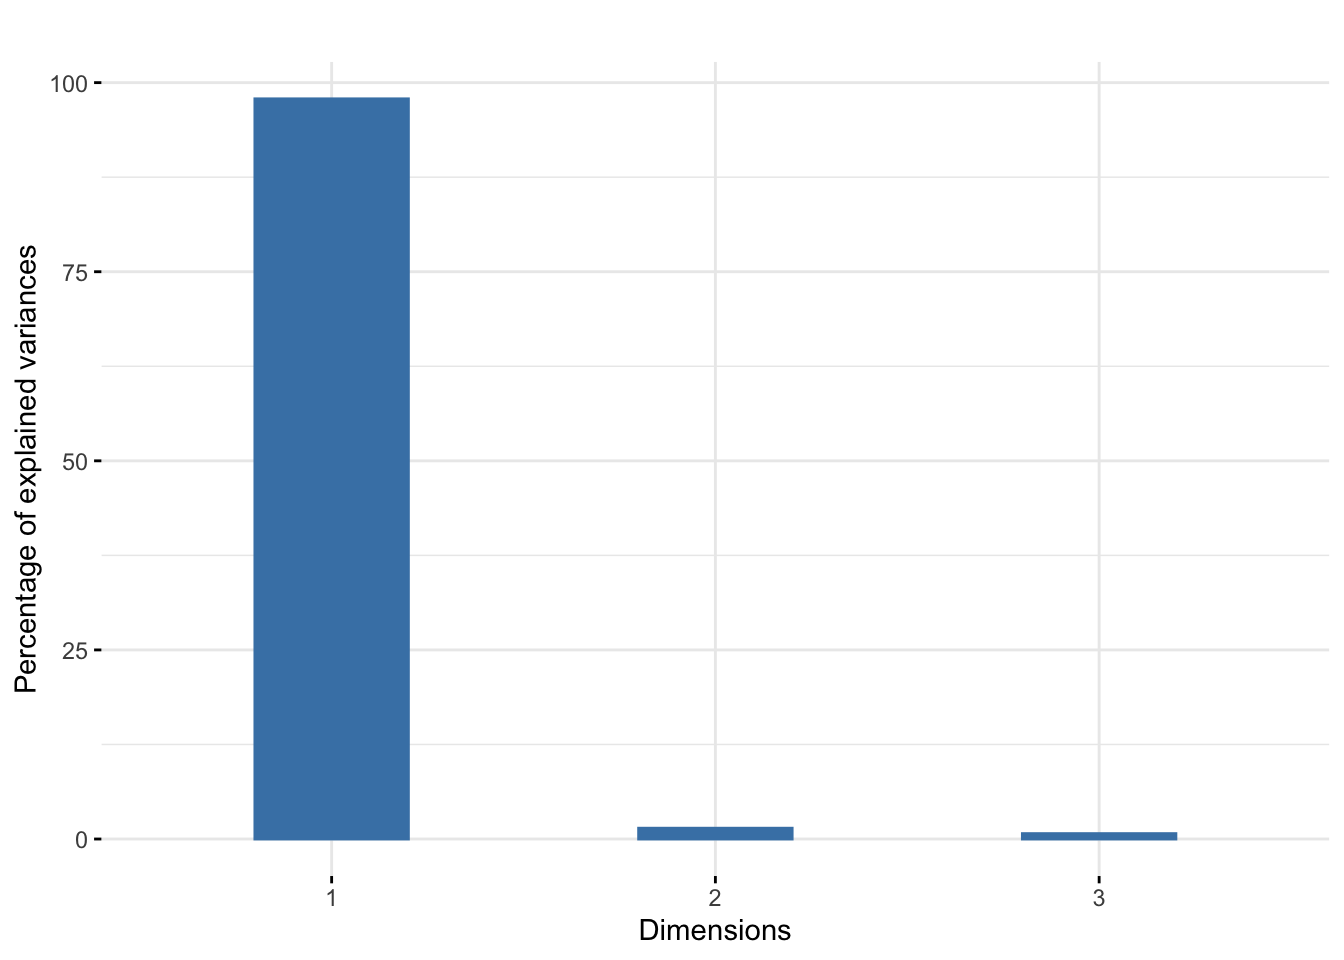
\includegraphics{Chapter4_files/figure-latex/unnamed-chunk-35-1.pdf}

\begin{Shaded}
\begin{Highlighting}[]
\CommentTok{#data after square root transformation}
\KeywordTok{ggplot}\NormalTok{(simdat2, }\KeywordTok{aes}\NormalTok{(}\DataTypeTok{x =}\NormalTok{ lambda, }\DataTypeTok{y =} \KeywordTok{sqrt}\NormalTok{(y))) }\OperatorTok{+}
\StringTok{  }\KeywordTok{geom_beeswarm}\NormalTok{(}\DataTypeTok{alpha =} \FloatTok{0.6}\NormalTok{, }\DataTypeTok{color =} \StringTok{"purple"}\NormalTok{)}
\end{Highlighting}
\end{Shaded}

\includegraphics{Chapter4_files/figure-latex/unnamed-chunk-35-2.pdf}

Now Using the gamma-Poisson distribution and and plotting the 95\%
confidence intervals around the mean.

\begin{Shaded}
\begin{Highlighting}[]
\NormalTok{muvalues =}\StringTok{ }\DecValTok{2}\OperatorTok{^}\KeywordTok{seq}\NormalTok{(}\DecValTok{0}\NormalTok{, }\DecValTok{10}\NormalTok{, }\DataTypeTok{by =} \DecValTok{1}\NormalTok{)}
\NormalTok{simgp =}\StringTok{ }\KeywordTok{lapply}\NormalTok{(muvalues, }\ControlFlowTok{function}\NormalTok{(mu) \{}
\NormalTok{  u =}\StringTok{ }\KeywordTok{rnbinom}\NormalTok{(}\DataTypeTok{n =} \FloatTok{1e4}\NormalTok{, }\DataTypeTok{mu =}\NormalTok{ mu, }\DataTypeTok{size =} \DecValTok{4}\NormalTok{)}
  \KeywordTok{tibble}\NormalTok{(}\DataTypeTok{mean =} \KeywordTok{mean}\NormalTok{(u), }\DataTypeTok{sd =} \KeywordTok{sd}\NormalTok{(u),}
         \DataTypeTok{lower =} \KeywordTok{quantile}\NormalTok{(u, }\FloatTok{0.025}\NormalTok{),}
         \DataTypeTok{upper =} \KeywordTok{quantile}\NormalTok{(u, }\FloatTok{0.975}\NormalTok{),}
         \DataTypeTok{mu =}\NormalTok{ mu)}
\NormalTok{  \} ) }\OperatorTok\StringTok{ }\NormalTok{bind_rows}
\KeywordTok{head}\NormalTok{(}\KeywordTok{as.data.frame}\NormalTok{(simgp), }\DecValTok{2}\NormalTok{)}
\end{Highlighting}
\end{Shaded}

\begin{verbatim}
##     mean       sd lower upper mu
## 1 1.0043 1.130048     0     4  1
## 2 2.0171 1.711286     0     6  2
\end{verbatim}

\begin{Shaded}
\begin{Highlighting}[]
\KeywordTok{ggplot}\NormalTok{(simgp, }\KeywordTok{aes}\NormalTok{(}\DataTypeTok{x =}\NormalTok{ mu, }\DataTypeTok{y =}\NormalTok{ mean, }\DataTypeTok{ymin =}\NormalTok{ lower, }\DataTypeTok{ymax =}\NormalTok{ upper)) }\OperatorTok{+}
\StringTok{  }\KeywordTok{geom_point}\NormalTok{() }\OperatorTok{+}\StringTok{ }\KeywordTok{geom_errorbar}\NormalTok{()}
\end{Highlighting}
\end{Shaded}

\includegraphics{Chapter4_files/figure-latex/unnamed-chunk-36-1.pdf} To
transform these data to normalize their standard deviation, divide the
values that correspond to mu{[}1{]} (and which are centered around
simgp\(mean[1]) by their standard deviation simgp\)sd{[}1{]}, the values
that correspond to mu{[}2{]} (and which are centered around
simgp\(mean[2]) by their standard deviation simgp\)sd{[}2{]}, and so on,
then the resulting values will have, by construction, a standard
deviation (and thus variance) of 1.

\begin{Shaded}
\begin{Highlighting}[]
\NormalTok{simgp =}\StringTok{ }\KeywordTok{mutate}\NormalTok{(simgp,}
  \DataTypeTok{slopes =} \DecValTok{1} \OperatorTok{/}\StringTok{ }\NormalTok{sd,}
  \DataTypeTok{trsf   =} \KeywordTok{cumsum}\NormalTok{(slopes }\OperatorTok{*}\StringTok{ }\NormalTok{mean))}
\KeywordTok{ggplot}\NormalTok{(simgp, }\KeywordTok{aes}\NormalTok{(}\DataTypeTok{x =}\NormalTok{ mean, }\DataTypeTok{y =}\NormalTok{ trsf)) }\OperatorTok{+}
\StringTok{  }\KeywordTok{geom_point}\NormalTok{() }\OperatorTok{+}\StringTok{ }\KeywordTok{geom_line}\NormalTok{() }\OperatorTok{+}\StringTok{ }\KeywordTok{xlab}\NormalTok{(}\StringTok{""}\NormalTok{)}
\end{Highlighting}
\end{Shaded}

\includegraphics{Chapter4_files/figure-latex/unnamed-chunk-37-1.pdf}

\#\#\#\#\#Exercises

\#\#Excersise 1 The EM algorithm step by step Model the Myst.rds dataset
as a mixture of two normal distributions (A and B) with unknown means
and standard deviations.

\begin{Shaded}
\begin{Highlighting}[]
\NormalTok{yvar =}\StringTok{ }\KeywordTok{readRDS}\NormalTok{(}\KeywordTok{here}\NormalTok{(}\StringTok{"Book"}\NormalTok{,}\StringTok{"data"}\NormalTok{,}\StringTok{"Myst.rds"}\NormalTok{))}\OperatorTok{$}\NormalTok{yvar}
\KeywordTok{ggplot}\NormalTok{(}\KeywordTok{tibble}\NormalTok{(yvar), }\KeywordTok{aes}\NormalTok{(}\DataTypeTok{x =}\NormalTok{ yvar)) }\OperatorTok{+}\StringTok{ }\KeywordTok{geom_histogram}\NormalTok{(}\DataTypeTok{binwidth=}\FloatTok{0.025}\NormalTok{)}
\end{Highlighting}
\end{Shaded}

\includegraphics{Chapter4_files/figure-latex/unnamed-chunk-38-1.pdf}

\begin{Shaded}
\begin{Highlighting}[]
\KeywordTok{str}\NormalTok{(yvar)}
\end{Highlighting}
\end{Shaded}

\begin{verbatim}
##  num [1:1800] 0.3038 0.0596 -0.0204 0.1849 0.2842 ...
\end{verbatim}

Create the Distributions with the code chunck below.

\begin{Shaded}
\begin{Highlighting}[]
\CommentTok{#First, simulate a random uniform distribution with the length of yvar (1800) yielding entry probabilities of the data points of the component}
\NormalTok{pA =}\StringTok{ }\KeywordTok{runif}\NormalTok{(}\KeywordTok{length}\NormalTok{(yvar))}
\CommentTok{#Make complementary propabilities of pA}
\NormalTok{pB =}\StringTok{ }\DecValTok{1} \OperatorTok{-}\StringTok{ }\NormalTok{pA}
\CommentTok{#housekeeping variables: iter counts over the iterations of the EM algorithm; loglik stores the current log-likelihood; delta stores the change in the log-likelihood from the previous iteration to the current one. We also define the parameters tolerance, miniter and maxiter of the algorithm.}

\NormalTok{iter =}\StringTok{ }\DecValTok{0}
\NormalTok{loglik =}\StringTok{ }\OperatorTok{-}\OtherTok{Inf}
\NormalTok{delta =}\StringTok{ }\OperatorTok{+}\OtherTok{Inf}
\NormalTok{tolerance =}\StringTok{ }\FloatTok{1e-3}
\NormalTok{miniter =}\StringTok{ }\DecValTok{50}\NormalTok{; maxiter =}\StringTok{ }\DecValTok{1000}
\ControlFlowTok{while}\NormalTok{((delta }\OperatorTok{>}\StringTok{ }\NormalTok{tolerance) }\OperatorTok{&&}\StringTok{ }\NormalTok{(iter }\OperatorTok{<=}\StringTok{ }\NormalTok{maxiter) }\OperatorTok{||}\StringTok{ }\NormalTok{(iter }\OperatorTok{<}\StringTok{ }\NormalTok{miniter)) \{}
  \CommentTok{#Provide an initial guess of the expected parameters }
\NormalTok{  lambda =}\StringTok{ }\KeywordTok{mean}\NormalTok{(pA)}
\NormalTok{  muA =}\StringTok{ }\KeywordTok{weighted.mean}\NormalTok{(yvar, pA)}
\NormalTok{  muB =}\StringTok{ }\KeywordTok{weighted.mean}\NormalTok{(yvar, pB)}
\NormalTok{  sdA =}\StringTok{ }\KeywordTok{sqrt}\NormalTok{(}\KeywordTok{weighted.mean}\NormalTok{((yvar }\OperatorTok{-}\StringTok{ }\NormalTok{muA)}\OperatorTok{^}\DecValTok{2}\NormalTok{, pA))}
\NormalTok{  sdB =}\StringTok{ }\KeywordTok{sqrt}\NormalTok{(}\KeywordTok{weighted.mean}\NormalTok{((yvar }\OperatorTok{-}\StringTok{ }\NormalTok{muB)}\OperatorTok{^}\DecValTok{2}\NormalTok{, pB))}

\NormalTok{  phiA =}\StringTok{ }\KeywordTok{dnorm}\NormalTok{(yvar, }\DataTypeTok{mean =}\NormalTok{ muA, }\DataTypeTok{sd =}\NormalTok{ sdA)}
\NormalTok{  phiB =}\StringTok{ }\KeywordTok{dnorm}\NormalTok{(yvar, }\DataTypeTok{mean =}\NormalTok{ muB, }\DataTypeTok{sd =}\NormalTok{ sdB)}
\NormalTok{  pA   =}\StringTok{ }\NormalTok{lambda }\OperatorTok{*}\StringTok{ }\NormalTok{phiA}
\NormalTok{  pB   =}\StringTok{ }\NormalTok{(}\DecValTok{1} \OperatorTok{-}\StringTok{ }\NormalTok{lambda) }\OperatorTok{*}\StringTok{ }\NormalTok{phiB}
\NormalTok{  ptot =}\StringTok{ }\NormalTok{pA }\OperatorTok{+}\StringTok{ }\NormalTok{pB}
\NormalTok{  pA   =}\StringTok{ }\NormalTok{pA }\OperatorTok{/}\StringTok{ }\NormalTok{ptot}
\NormalTok{  pB   =}\StringTok{ }\NormalTok{pB }\OperatorTok{/}\StringTok{ }\NormalTok{ptot}

\NormalTok{  loglikOld =}\StringTok{ }\NormalTok{loglik}
\NormalTok{  loglik =}\StringTok{ }\KeywordTok{sum}\NormalTok{(}\KeywordTok{log}\NormalTok{(pA))}
\NormalTok{  delta =}\StringTok{ }\KeywordTok{abs}\NormalTok{(loglikOld }\OperatorTok{-}\StringTok{ }\NormalTok{loglik)}
\NormalTok{  iter =}\StringTok{ }\NormalTok{iter }\OperatorTok{+}\StringTok{ }\DecValTok{1}
\NormalTok{\}}
\NormalTok{param =}\StringTok{ }\KeywordTok{tibble}\NormalTok{(}\DataTypeTok{group =} \KeywordTok{c}\NormalTok{(}\StringTok{"A"}\NormalTok{,}\StringTok{"B"}\NormalTok{), }\DataTypeTok{mean =} \KeywordTok{c}\NormalTok{(muA,muB), }\DataTypeTok{sd =} \KeywordTok{c}\NormalTok{(sdA,sdB))}
\NormalTok{param}
\end{Highlighting}
\end{Shaded}

\begin{verbatim}
## # A tibble: 2 x 3
##   group   mean     sd
##   <chr>  <dbl>  <dbl>
## 1 A      0.147 0.150 
## 2 B     -0.169 0.0983
\end{verbatim}

\begin{Shaded}
\begin{Highlighting}[]
\NormalTok{iter}
\end{Highlighting}
\end{Shaded}

\begin{verbatim}
## [1] 359
\end{verbatim}

\begin{enumerate}
\def\labelenumi{\alph{enumi}.}
\tightlist
\item
  Which lines correspond to the E-step, which to the M-step?
\end{enumerate}

Algorithm for EM is i. Given a set of incomplete data, consider a set of
starting parameters. ii. Expectation step (E -- step): Using the
observed available data of the dataset, estimate (guess) the values of
the missing data.This is represented in the code as; lambda = mean(pA)
\textgreater{}muA = weighted.mean(yvar, pA) \textgreater{}muB =
weighted.mean(yvar, pB) \textgreater{}sdA = sqrt(weighted.mean((yvar -
muA)\^{}2, pA)) \textgreater{}sdB = sqrt(weighted.mean((yvar -
muB)\^{}2, pB))

\begin{enumerate}
\def\labelenumi{\roman{enumi}.}
\setcounter{enumi}{2}
\tightlist
\item
  Maximization step (M -- step): Complete data generated after the
  expectation (E) step is used in order to update the parameters. This
  is represented in the code as; \textgreater{} phiA = dnorm(yvar, mean
  = muA, sd = sdA) \textgreater{} phiB = dnorm(yvar, mean = muB, sd =
  sdB) \textgreater{} pA = lambda * phiA \textgreater{} pB = (1 -
  lambda) * phiB \textgreater{} ptot = pA + pB \textgreater{}\\
  \textgreater{} pA = pA / ptot \textgreater{} pB = pB / ptot
\end{enumerate}

\begin{enumerate}
\def\labelenumi{\alph{enumi}.}
\setcounter{enumi}{1}
\tightlist
\item
  What does the M-step do, what does the E-step do? E-step: Using the
  observed available data of the dataset, estimate (guess) the values of
  the missing data
\end{enumerate}

Maximization step (M -- step): Complete data generated after the
expectation (E) step is used in order to update the parameters.

\begin{enumerate}
\def\labelenumi{\alph{enumi}.}
\setcounter{enumi}{2}
\tightlist
\item
  What is the role of the algorithm arguments tolerance, miniter and
  maxiter? Tolerance argument the minimum difference between estimated
  log-likelihood. A diiferent \textless{}= this indicaes vonvergence and
  termination of iteration. Miniter is the least number of times that we
  can interate between the E and M steps. Maxiter is the largest
  threashold for iteration between the E and M steps.
\end{enumerate}

d.Why do we need to compute loglik? loglik estimation is relevant for
determining convergence. It is used in estimating delta which is in turn
compared with the predefined tolerance argument for assessing
convergence.

\begin{enumerate}
\def\labelenumi{\alph{enumi}.}
\setcounter{enumi}{4}
\tightlist
\item
  Compare the result to the output of the normalmixEM function from the
  mixtools package.
\end{enumerate}

\begin{Shaded}
\begin{Highlighting}[]
\NormalTok{mixtoolsQ <-}\StringTok{ }\KeywordTok{normalmixEM}\NormalTok{(yvar, }\DataTypeTok{k=}\DecValTok{2}\NormalTok{,}\DataTypeTok{lambda=}\KeywordTok{c}\NormalTok{(}\FloatTok{0.5}\NormalTok{,}\FloatTok{0.5}\NormalTok{), }\DataTypeTok{mu=}\KeywordTok{c}\NormalTok{(muA,muB), }\DataTypeTok{sigma=}\KeywordTok{c}\NormalTok{(sdA,sdB),  }\DataTypeTok{maxit=}\DecValTok{1000}\NormalTok{)}
\end{Highlighting}
\end{Shaded}

\begin{verbatim}
## number of iterations= 149
\end{verbatim}

\begin{Shaded}
\begin{Highlighting}[]
\NormalTok{mixtoolsQ}\OperatorTok{$}\NormalTok{mu}
\end{Highlighting}
\end{Shaded}

\begin{verbatim}
## [1]  0.1473373 -0.1693509
\end{verbatim}

\begin{Shaded}
\begin{Highlighting}[]
\NormalTok{mixtoolsQ}\OperatorTok{$}\NormalTok{sigma}
\end{Highlighting}
\end{Shaded}

\begin{verbatim}
## [1] 0.14977994 0.09826952
\end{verbatim}

\begin{Shaded}
\begin{Highlighting}[]
\NormalTok{mixtoolsQ}\OperatorTok{$}\NormalTok{loglik}
\end{Highlighting}
\end{Shaded}

\begin{verbatim}
## [1] 417.2218
\end{verbatim}

The results are similar. However the normalmixEM function acheives the
optimal loglik at a constantly lower iteration (149).

\#\#Excersise 2 Compare the theoretical values of the gamma-Poisson
distribution with parameters given by the estimates in ofit\$par in
Section 4.4.3 to the data used for the estimation using a QQ-plot.

\begin{Shaded}
\begin{Highlighting}[]
\CommentTok{#Obtain quantiles of the two heirachy simulated data (gp). But first use ppoints() to find the ordinates}
\NormalTok{ordinates=}\StringTok{ }\KeywordTok{ppoints}\NormalTok{(}\DecValTok{1000}\NormalTok{)}
\NormalTok{quant_raw=}\KeywordTok{quantile}\NormalTok{(gp,ordinates)}

\CommentTok{#Generate theoretical values of the gamma-Poisson distributions (using parameters of ofit$par) and obtain their quantiles  with the same ordinates}

\NormalTok{gamma_pois =}\StringTok{ }\KeywordTok{qnbinom}\NormalTok{(}\DataTypeTok{p=}\NormalTok{ordinates,}\DataTypeTok{size=}\NormalTok{ofit}\OperatorTok{$}\NormalTok{par[[}\DecValTok{1}\NormalTok{]], }\DataTypeTok{prob=}\NormalTok{ofit}\OperatorTok{$}\NormalTok{par[[}\DecValTok{2}\NormalTok{]])}
\NormalTok{quant_gamma_pois=}\KeywordTok{quantile}\NormalTok{(gamma_pois,ordinates)}

\CommentTok{# plot the two for comparison}
\KeywordTok{plot}\NormalTok{(quant_raw,quant_gamma_pois)}
\KeywordTok{abline}\NormalTok{(}\DataTypeTok{a =}\DecValTok{0}\NormalTok{, }\DataTypeTok{b=}\DecValTok{1}\NormalTok{, }\DataTypeTok{col=}\StringTok{"red"}\NormalTok{)}
\end{Highlighting}
\end{Shaded}

\includegraphics{Chapter4_files/figure-latex/unnamed-chunk-40-1.pdf}

There is a high similarity among both datasets.

\#\#Excersice 3

\begin{enumerate}
\def\labelenumi{\alph{enumi})}
\tightlist
\item
  First, plot the data and try to guess how the points were generated.
\end{enumerate}

\begin{Shaded}
\begin{Highlighting}[]
\CommentTok{#load data, view and plot plot NPreg data}

\KeywordTok{data}\NormalTok{(}\StringTok{"NPreg"}\NormalTok{)}
\KeywordTok{head}\NormalTok{(NPreg)}
\end{Highlighting}
\end{Shaded}

\begin{verbatim}
##          x        yn yp yb class id1 id2
## 1 4.176633 22.380379  4  0     1   1   1
## 2 1.201631  5.111575  3  0     1   1   1
## 3 2.295006 13.251058  9  0     1   2   1
## 4 5.965868 30.285240  3  1     1   2   1
## 5 2.358083 14.764508  4  0     1   3   2
## 6 7.637061 42.833760  1  1     1   3   2
\end{verbatim}

\begin{Shaded}
\begin{Highlighting}[]
\KeywordTok{summary}\NormalTok{(NPreg)}
\end{Highlighting}
\end{Shaded}

\begin{verbatim}
##        x                 yn               yp               yb       
##  Min.   :0.06295   Min.   :-1.482   Min.   : 0.000   Min.   :0.000  
##  1st Qu.:2.67892   1st Qu.:20.489   1st Qu.: 2.000   1st Qu.:0.000  
##  Median :5.07820   Median :30.933   Median : 4.000   Median :0.000  
##  Mean   :5.03078   Mean   :28.607   Mean   : 3.955   Mean   :0.475  
##  3rd Qu.:7.37686   3rd Qu.:38.322   3rd Qu.: 5.000   3rd Qu.:1.000  
##  Max.   :9.89474   Max.   :53.487   Max.   :12.000   Max.   :1.000  
##                                                                     
##      class          id1           id2     
##  Min.   :1.0   1      :  2   1      :  4  
##  1st Qu.:1.0   2      :  2   2      :  4  
##  Median :1.5   3      :  2   3      :  4  
##  Mean   :1.5   4      :  2   4      :  4  
##  3rd Qu.:2.0   5      :  2   5      :  4  
##  Max.   :2.0   6      :  2   6      :  4  
##                (Other):188   (Other):176
\end{verbatim}

\begin{Shaded}
\begin{Highlighting}[]
\CommentTok{#There is an independent varianble (x) and three dependent variables following the Normal(yn), Poisson(yp) and Binomial(yb) Regression and two  classes.}

\KeywordTok{ggplot}\NormalTok{(NPreg, }\KeywordTok{aes}\NormalTok{(}\DataTypeTok{x =}\NormalTok{ x, }\DataTypeTok{y =}\NormalTok{ yn, }\DataTypeTok{color=}\KeywordTok{as.factor}\NormalTok{(class))) }\OperatorTok{+}\StringTok{ }\KeywordTok{geom_point}\NormalTok{()}
\end{Highlighting}
\end{Shaded}

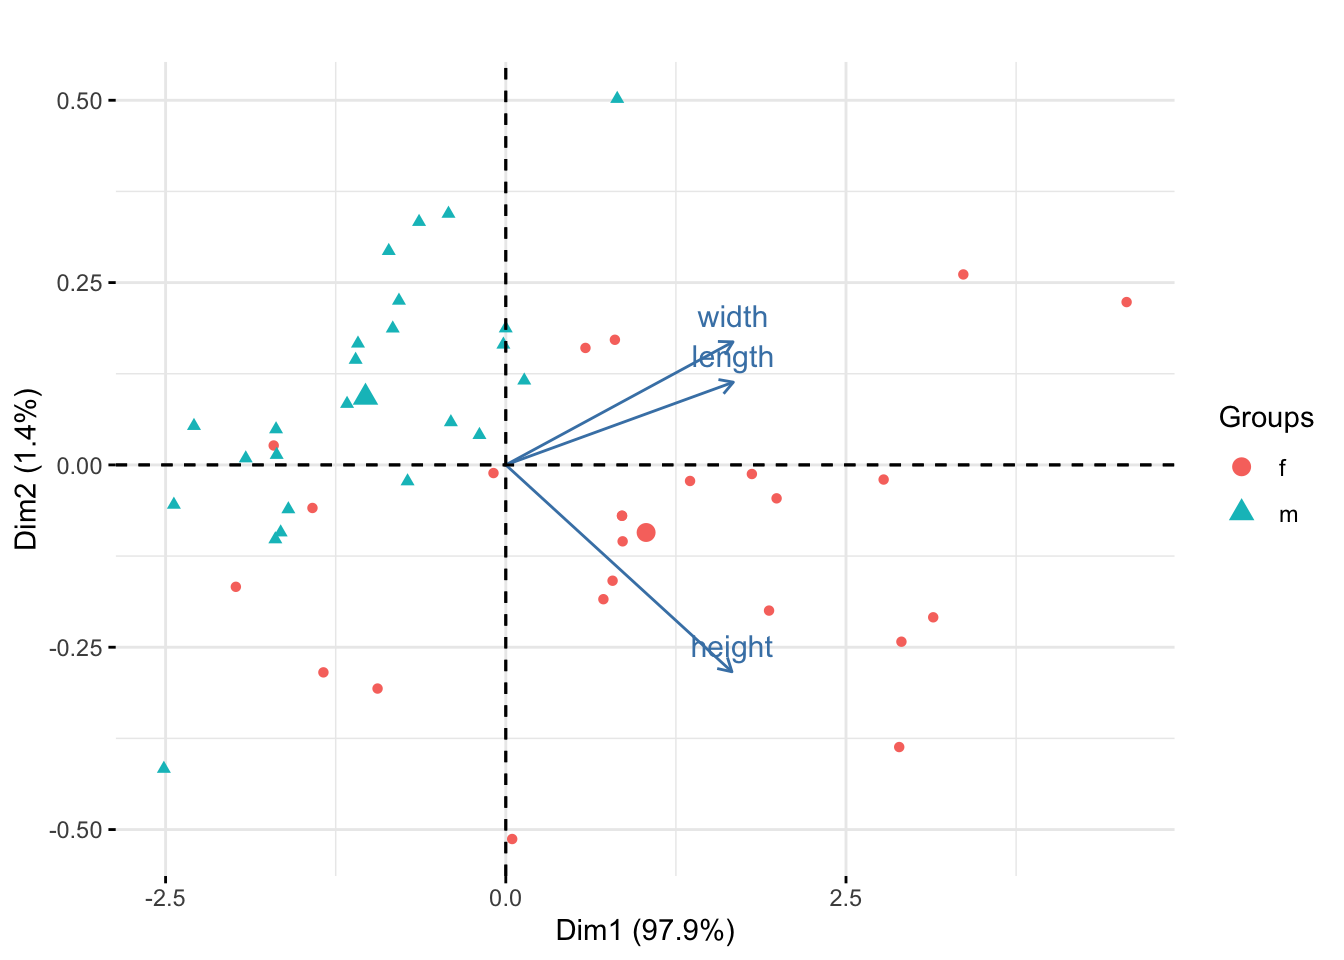
\includegraphics{Chapter4_files/figure-latex/unnamed-chunk-41-1.pdf}

\begin{Shaded}
\begin{Highlighting}[]
\KeywordTok{ggplot}\NormalTok{(NPreg, }\KeywordTok{aes}\NormalTok{(}\DataTypeTok{x =}\NormalTok{ x, }\DataTypeTok{y =}\NormalTok{ yp, }\DataTypeTok{color=}\KeywordTok{as.factor}\NormalTok{(class))) }\OperatorTok{+}\StringTok{ }\KeywordTok{geom_point}\NormalTok{()}
\end{Highlighting}
\end{Shaded}

\includegraphics{Chapter4_files/figure-latex/unnamed-chunk-41-2.pdf}

\begin{Shaded}
\begin{Highlighting}[]
\KeywordTok{ggplot}\NormalTok{(NPreg, }\KeywordTok{aes}\NormalTok{(}\DataTypeTok{x =}\NormalTok{ x, }\DataTypeTok{y =}\NormalTok{ yb, }\DataTypeTok{color=}\KeywordTok{as.factor}\NormalTok{(class))) }\OperatorTok{+}\StringTok{ }\KeywordTok{geom_point}\NormalTok{()}
\end{Highlighting}
\end{Shaded}

\includegraphics{Chapter4_files/figure-latex/unnamed-chunk-41-3.pdf}

Of all the plots, the normal regression (yn) is easily distiguishable by
class. Class 1 seems to follow a linear regression while class two
follows a non-linear (possibly quadratic) regression.

\begin{enumerate}
\def\labelenumi{\alph{enumi}.}
\setcounter{enumi}{1}
\tightlist
\item
  Fit a two component mixture model using the commands;
\end{enumerate}

\begin{Shaded}
\begin{Highlighting}[]
\NormalTok{m1 =}\StringTok{ }\KeywordTok{flexmix}\NormalTok{(yn }\OperatorTok{~}\StringTok{ }\NormalTok{x }\OperatorTok{+}\StringTok{ }\KeywordTok{I}\NormalTok{(x}\OperatorTok{^}\DecValTok{2}\NormalTok{), }\DataTypeTok{data =}\NormalTok{ NPreg, }\DataTypeTok{k =} \DecValTok{2}\NormalTok{)}

\CommentTok{#this is a two component model. We can easily observe the cluster sizes, convergence iterations by running the object. More info can be obtained by summary}
\NormalTok{m1}
\end{Highlighting}
\end{Shaded}

\begin{verbatim}
## 
## Call:
## flexmix(formula = yn ~ x + I(x^2), data = NPreg, k = 2)
## 
## Cluster sizes:
##   1   2 
## 100 100 
## 
## convergence after 15 iterations
\end{verbatim}

\begin{Shaded}
\begin{Highlighting}[]
\KeywordTok{summary}\NormalTok{(m1)}
\end{Highlighting}
\end{Shaded}

\begin{verbatim}
## 
## Call:
## flexmix(formula = yn ~ x + I(x^2), data = NPreg, k = 2)
## 
##        prior size post>0 ratio
## Comp.1 0.494  100    145 0.690
## Comp.2 0.506  100    141 0.709
## 
## 'log Lik.' -642.5453 (df=9)
## AIC: 1303.091   BIC: 1332.775
\end{verbatim}

\begin{Shaded}
\begin{Highlighting}[]
\CommentTok{#We can also observe the associated parameter of the componets by running parameters() and selecting the appropraite component}
\end{Highlighting}
\end{Shaded}

c.Look at the estimated parameters of the mixture components and make a
truth table that cross-classifies true classes versus cluster
memberships. What does the summary of the object m1 show us?

\begin{Shaded}
\begin{Highlighting}[]
\KeywordTok{parameters}\NormalTok{(m1, }\DataTypeTok{component =} \DecValTok{1}\NormalTok{)}
\end{Highlighting}
\end{Shaded}

\begin{verbatim}
##                       Comp.1
## coef.(Intercept) -0.20959655
## coef.x            4.81774867
## coef.I(x^2)       0.03616097
## sigma             3.47652037
\end{verbatim}

\begin{Shaded}
\begin{Highlighting}[]
\KeywordTok{parameters}\NormalTok{(m1, }\DataTypeTok{component =} \DecValTok{2}\NormalTok{)}
\end{Highlighting}
\end{Shaded}

\begin{verbatim}
##                      Comp.2
## coef.(Intercept) 14.7171140
## coef.x            9.8466333
## coef.I(x^2)      -0.9683531
## sigma             3.4796257
\end{verbatim}

\begin{Shaded}
\begin{Highlighting}[]
\CommentTok{# we can now create a contingency table using the class and clusters}
\KeywordTok{table}\NormalTok{(NPreg}\OperatorTok{$}\NormalTok{class, }\KeywordTok{clusters}\NormalTok{(m1))}
\end{Highlighting}
\end{Shaded}

\begin{verbatim}
##    
##      1  2
##   1 95  5
##   2  5 95
\end{verbatim}

\begin{Shaded}
\begin{Highlighting}[]
\KeywordTok{summary}\NormalTok{(m1)}
\end{Highlighting}
\end{Shaded}

\begin{verbatim}
## 
## Call:
## flexmix(formula = yn ~ x + I(x^2), data = NPreg, k = 2)
## 
##        prior size post>0 ratio
## Comp.1 0.494  100    145 0.690
## Comp.2 0.506  100    141 0.709
## 
## 'log Lik.' -642.5453 (df=9)
## AIC: 1303.091   BIC: 1332.775
\end{verbatim}

The summary provides information on the log Lik (-642.5453) degreed of
freedom (df=9) AIC: 1303.091 and BIC: 1332.776. The prior and size
poterior of both classes are also indicated.

\begin{enumerate}
\def\labelenumi{\alph{enumi}.}
\setcounter{enumi}{3}
\tightlist
\item
  Plot the data again, this time coloring each point according to its
  estimated class.
\end{enumerate}

\begin{Shaded}
\begin{Highlighting}[]
\KeywordTok{ggplot}\NormalTok{(NPreg, }\KeywordTok{aes}\NormalTok{(}\DataTypeTok{x =}\NormalTok{ x, }\DataTypeTok{y =}\NormalTok{ yn, }\DataTypeTok{group =}\NormalTok{ class)) }\OperatorTok{+}
\StringTok{   }\KeywordTok{geom_point}\NormalTok{(}\KeywordTok{aes}\NormalTok{(}\DataTypeTok{colour =} \KeywordTok{as.factor}\NormalTok{(m1}\OperatorTok{@}\NormalTok{cluster), }\DataTypeTok{shape =} \KeywordTok{factor}\NormalTok{(class)))}
\end{Highlighting}
\end{Shaded}

\includegraphics{Chapter4_files/figure-latex/unnamed-chunk-44-1.pdf}

\hypertarget{exercise-4}{%
\section{Exercise 4}\label{exercise-4}}

Other hierarchical noise models: Find two papers that explore the use of
other infite mixtures for modeling molecular biology technological
variation.

\begin{enumerate}
\def\labelenumi{\arabic{enumi}.}
\item
  Yau, C., Papaspiliopoulos, O., Roberts, G.O. and Holmes, C., 2011.
  Bayesian non‐parametric hidden Markov models with applications in
  genomics. Journal of the Royal Statistical Society: Series B
  (Statistical Methodology), 73(1), pp.37-57.
\item
  Dang, T. and Kishino, H., 2019. Stochastic variational inference for
  Bayesian phylogenetics: A case of CAT model. Molecular biology and
  evolution, 36(4), pp.825-833.
\end{enumerate}


\end{document}
